\begin{refsection}
\chapter{Теоретичні основи лапароскопічної хірургії печінки}

\section{Історія розвитку методики}
\subsection{Перший досвід}
Мініінвазивні втручання радикально змінили хірургічну практику за останні три десятиріччя. Їх поява призвела до суттєвого покращення результатів за рахунок зменшення частоти післяопераційних ускладненнь, тривалості госпіталізації та співвідношення вартості до еффективності лікування.  Ці зміни торкнулись багатьох хірургічних спеціальностей, включаючи колоректальну хірургію, урологію, гінекологію та торокальну хірургію. Природньо, що зацікавленість хірургів в лапароскопічному доступі швидко розповсюдилась на гепатобіліарні втручання, спроби виконання яких в лапароскопічному варіанті було розпочато в 1987 році із першої лапароскопічної холецистектомії \cite{Litynski}. 

Для лікування уражень печінки лапароскопія була вперше впроваджена на початку 90х. На відміну від інших галузей, в печінковій хірургії лапароскопія зіткнулась із багатьма технічними перешкодами, пов'язаними із складною внутрішньою будовою та вразливою, схильною до кровотеч паренхімою печінки. Проте переваги лапароскопічного доступу, такі як покращена візуалізація, та зменшення післяопераційних ускладненнь, надали стимул для розвитку лапароскопічних резекцій печінки та здолання цих перешкод (\acrshort{llr}). 

Перші резекції печінки в лапароскопічному варіанті були виконані в 1991 році Reich H. \cite{Reich1991a} та  в 1992 Katkhouda N. \cite{Katkhouda1992} та Gagner M. \cite{GAGNER1992}. Ці операції були крайовими резекціями невеликих, переважно доброякісних, новоутворень. Невдовзі стало зрозуміло, що результати лапароскопічних операцій порівняні із традиційними відкритими втручаннями а \acrshort{llr} є безпечним та ефективним методом лікування. Відтоді \acrshort{llr} стала потенційною альтернативою відкритій резекції печінки (\acrshort{olr}). 

На початковому етапі розвиток методики був повільним, і наступні декілька років після першої згадки про \acrshort{llr} публікації містили лише опис поодиноких випадків атипових резекцій \cite{Klotz1993, Cunningham1995}. Перша анатомічна лапароскопічна лівобічна латеральна секцієектомія(\acrshort{llls}) виконана в 1996 році \cite{Azagra1996}  відновила інтерес до \acrshort{llr}  \cite{Hashizume1995}.  Із накопиченням досвіду покази до \acrshort{llr} були розширені до гемігепатектомій, складних сегментектомій, трисекцієектомій та навіть донорських резекцій при трансплантації печінки від живого донора \cite{Dagher2009, Cherqui2002, Jia2018}. 

\subsection{Погоджувальні конференції}

Від моменту виконання першої \acrshort{llr} кількість публікацій присвячених темі щорічно прогресивно збільшується (Рис. \ref{fig:PubMed_publications}). Стимулом до цього є посітйне вдосконалення ендохірургічного обладнання та хірургічної техніки.

Набутий досвід створив необхідність оцінки хірургічною спільнотою безпеки, відтворюваності та онкологічної ефективності \acrshort{llr}. Для вирішення цих завданнь та створення клінічних рекомендацій стосовно застосування \acrshort{llr} було  проведено декілька погоджувальних конференцій, висновки яких відображують процес становлення лапароскопічного методу та зміну відношення до нього хірургічного загалу. 

\begin{figure}[h]
\caption{Динаміка кількості публікацій в PubMed по запиту "laparosopic liver resection" по роках \cite{Hashizume1995}}
\centering
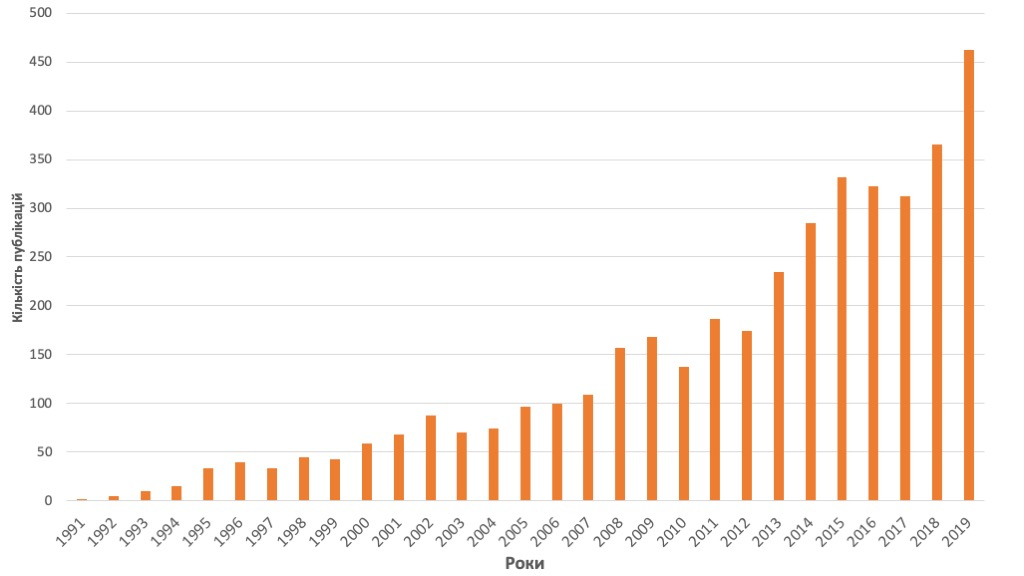
\includegraphics[width=0.9\textwidth]{Illustrations/Chapter_01/PubMed_publications.jpg}
\label{fig:PubMed_publications}
\end{figure}

\subsubsection{Перша погоджувальна конференція} 

Перша погоджувальна конференція відбулась в Луізвілі в листопаді 2008 року за участі 45 міжнародних експертів з гепатобіліарної хірургії. \cite{Buell2009}. За результатами обговорення до  \acrshort{llr} були віднесені чисто лапароскопічні, хенд-асистовані резекції печінки (\acrshort{hals}) та гибридні резекції печінки (\acrshort{hlr}) при яких початкова диссекція проводиться в лапароскопічному варіанті а розсічення паренхіми через мінілапаротомію. 

Прийнятними для видалення за допомогою \acrshort{llr} були визначені утворення, розміром менше 5 см, що розташовані в 2 - 6 сегментах печінки, а \acrshort{llls} було рекомендовано розглядати в якості стандартної практики. Також була показана принципова технічна можливість видалення новоутворень, локалізованих в будь яких сегментах печінки в лапароскопічному варіанті, проте обширні резекції печінки було рекомендовано зарезервувати за спеціалізованими гепатобіліарними центрами з великим досвідом як лапароскопічних втручаннь, так і резекційної хірургії печінки. 

Конверсію рекомендовано розглядати скоріше як необхідний крок для безпечного завершення складного втручання, ніж як ускладнення. Перед ургентною конверсією з приводу кровотечі хірург повинен докласти максимальних зусиль до зупинки кровотечі лапароскопічними методами. 

Вперше була показана можливість виконання донорського забору печінки при трансплантації від живого донора у дітей в лапароскопічному варіанті. Донорську \acrshort{llls} було оцінено, як експериментальну методику, що має великий потенціал але потребує детального вивчення. 

Загалом консенсус визначив \acrshort{llr} як безпечну альтернативу традиційним резекціям та рекомендував методику до подальшого вивчення та більш широкого впровадження досвідченими гепатобіліарними хірургами.

\subsubsection{Друга погоджувальна конференція} 

Друга погоджувальна конференція, яка відбулась в японському місті Моріока в жовтні 2014 році \cite{Kaneko2015}, була побудована за Цюріхсько-Датською моделлю, та включала в себе експертну панель з 43 досвідчених хірургів та 9 членів жюрі з 18 країн які оцінювали результати \acrshort{llr}. Для оцінки були запропоновані 17 запитаннь в категоріях переваги, ризики та технічні аспекти \acrshort{llr}. Доказова якість рекомендацій була оцінена за шкалою GRADE а ступінь розробки втручаннь за системою IDEAL \cite{Guyatt2008, McCulloch2009}. 

До малих резекцій (Minor resection) було віднести резекції 2 та меньше сегментів а до великих або обширних (Major resection) 3 та більше сегментів. Зважаючи на те, що технічна складність \acrshort{llls} та правобічної задньої або передньої секцієектомії в лапароскопічному варіанті значно відрізняються, резекції, до складу яких входять сегменти 7 або 8 було віднесено до технічно великих. 

За висновками експертного жюрі як малі так і великі \acrshort{llr} не гірші за відкриті в показниках операційної летальності, післяопераційних ускладненнь, чистоті резекційного краю, загальної виживаності, вартості операції та мають перевагу в більш короткому терміні перебування в стаціонарі, меншій крововтраті. Експерти погодились з тим, що результати лапароскопічних донорських заборів не відрізнялись від відкритих у високоспеціалізованих центрах. У якості додаткового висновку жюрі зазначило, що великі \acrshort{llr} вимагають високого рівню хірургічних навичок та тривалої кривої навчання.

Основними досягненнями конференції було по-перше визнання того, що  \acrshort{llr} за більшістю показників не поступаються, а за окремими показниками перевершують відкриті втручання, а по-друге рекомендація використовувати малі \acrshort{llr} в якості стандарту надання допомоги.

\subsubsection{Третя погоджувальна конференція та створення клінічних рекомендацій} 

Подальший еспотенціальний ріст кількості \acrshort{llr} призвів до того, що в лютому 2017 року в Саузхемптоні була проведена третя погоджувальна конференція яка мала на меті створення загальноєвропейських клінічних рекомендацій \cite{AbuHilal2017a}. В процесі підготовки було залучено експертну панель з 11 досвідчених гепатобіліарних хірургів, одна частина з яких мала досвід лише відкритих резекцій печінки а друга частина як відкритих так і \acrshort{llr}. Після аналітичного огляду 647 джерел, відібраних за допомогою критеріїв включення експертами були сформовані рекомендації в п'яти ключових напрямках: покази, відбір пацієнтів, види втручаннь, технічні особливості та імплементація.

Згідно з цими рекомендаціями \acrshort{llr} показані для лікування метахронних колоректальних метастазів та гепатоцеллюлярної карциноми.  Вони ассоційовані зі зниженням крововтрати, післяопераційного асциту, печінкової недостатності та терміну перебування в стаціонарі, порівняно із відкритими втручаннями при співставній тривалості операції, частоті R0 краю резекції та рівні рецидивів. Окрім того \acrshort{llr} показані для лікування доброякісної вогнищевої патології завдяки суттєвому зниженню післяопераційних ускладненнь, больового синдрому та терміну перебування в стаціонарі, що підтверджено на великих серіях пацієнтів, у тому числі із великими резекціями. Донорські гепатектомії не були визнані добре стандартизованими процедурами, та зарезервовані за високоспеціалізованими центрами.

Стосовно відбору пацієнтів, то \acrshort{llr} добре показали себе у хворих з вираженою коморбідністю та можуть бути рекомендовані для пацієнтів з ожирінням та пацієнтів старшого віку. Є данні, які свідчать про полегшення перебігу повторних (відкритих або лапароскопічних) резекцій печінки у пацієнтів, що вже перенесли \acrshort{llr}. Складні випадки з великими новоутвореннями (> 10 см) та близкістю до магістральних судин не є протипоказами до \acrshort{llr}, так як можуть бути виконані з аналогічною відкритим операціям  морбідністю.

Також в рекомнедаціях зазначено, що жодна з існуючих технік виконання \acrshort{llr} (\acrshort{hals}, \acrshort{hlr} або чисто лапароскопічна) не показала абсолютної переваги над іншими, проте вважається, що \acrshort{hals} та \acrshort{hlr} є перехідними до чисто лапароскопічної техніки. Те ж саме стосується й техніки транссекції паренхіми: краш-кламп, використання CUSA або інших хірургічних енергій визнано рівноцінними методами. 
   
Для диссекції портальних структур більшисть хірургів використовують ізольоване лігування, проте глісоновий підхід показав аналогічні результати. Для контролю кровотечі під час \acrshort{llr} рекомендовано використовувати лапароскопічний прийом Прінгла та анастезію з низьким центральним венозним тиском (\acrshort{cvp}). Факторами ризику конверсії на відкрите втручання є високий індекс маси тіла, розмір пухлини, локалізація ураження в постеролатеральних сегментах та цирроз. Перед виконанням ургентної конверсії рекомендовано досягти тимчасового гемостаза лапароскопічними методами.

Крива навчання малих \acrshort{llr} складає 60 випадків для хірурга, що має досвід відкритих резекцій печінки. Для великих \acrshort{llr} цей показник становить 55 операцій, при умові успішного проходження кривої для малих \acrshort{llr}. Впровадження \acrshort{llr} не повинно відбуватись в ізоляції від відкритої хірургії печінки. Для кожного спелізованого гепатобіліарного центру рекомендована наявність не менше двох хірургів, спеціалізованих на \acrshort{llr}.

Якщо послідовно проаналізувати висновки всіх погоджувальних конференцій стає зрозумілим, що методика \acrshort{llr} успішно пройшла крізь етапи розробки, первинної оцінки результатів та широкого впровадження базуючись на принципах доказової медицини. Чисельна кількість дослідженнь на великих групах пацієнтів \cite{Ciria2016b, Takahara2016, Berardi2017}, в тому числі два рандомізоаних клінічних дослідження \cite{Fretland2018b, Robles-Campos2019} свідчать про перевагу \acrshort{llr} над традиційними відкритими втручаннями в періопераційних показниках зі збереженням онкологічної ефективності. 

Усі види \acrshort{llr}, як великі так і малі, асоційовані зі зменшенням інтраопераційної крововтрати, післяопераційних ускладненнь та терміну перебування в стаціонарі та аналогічними показниками онкологічної результативності порівняно з віткритими втручаннями. Великі втручання та втручання на задніх сегментах пов'язані із більшою складністю та тривалістю операції, проте в експертних центрах можуть бути досягнуті периопераційні результати аналогічні малим \acrshort{llr}.


\section[Сучасні можливості]{Сучасні можливості лапароскопічної резекційної хірургії печінки}

\subsection{Анатомічні резекції печінки}
	
З моменту першої \acrshort{llr} можливості методу значно поширились за межі крайових резекцій новоутворень невеликого розміру. На данний момент показана доступність виконання в лапароскопічному варіанті абсолютно всіх видів анатомічних резекцій печінки при доброякісних та онкологічних пухлинах, включно навіть з операціями при хіларній холангіокарциномі. Найбільш часто вживані резекції, такі як \acrshort{llls}, лівобічна та правобічна гемігепатектомія та моносегментектомії є добре вивченими та стандартизованими процедурами, що дозволяє деяким спеціалізованим центрам \cite{Garbarino2019} виконувати до 80-90\% всіх резекцій печінки в лапароскопічному варіанті.

За об'ємом розрізняють малі (Minor) та великі або обширні (Major) резекції. До малих резекцій відносять моно- та бісегментектомії антеролатеральних сегменітв та ліву латеральну секцієектомію. До великих або обширних анатомічних \acrshort{llr} відностяь резекції при яких виляляють три або більше розташованих поруч сегмента. Класичними представниками великих резекцій є лівобічна та правобічна гемігепатектомії, правобічна передня та задня секцієектомії, мезогепатектомія.

\subsubsection{Лівобічна гемігепатектомія}

Лапароскопічна лівобічна гемігепатектомія (\acrshort{llhe}) показала себе як доступна, безпечна та ефективна процедура для пацієнтів, що мають новоутворення лівої долі печінки (Рис. \ref{fig:LeftLobe}). В ретроспективному порівняльному аналізі 62 \acrshort{llhe} та 118 відкритих лівобічних гемігепатектомій у пацієнтів з гепатоцеллюлярною карциномою (\acrshort{hcc}), внутрішньопечінковою холангіокарциномою (\acrshort{ihcc}) та деякими доброякісними новоутвореннями показано перевагу лапароскопічних втручаннь за рахунок зменшення крововтрати, часу до відновлення харчування та частоти важких ускладненнь з порівняними показниками виживаності у онкологічних хворих \cite{Cho2018b}.   

Міжнародне мультицентрове ретроспективне дослідження реузльтатів 82 \acrshort{llhe} \cite{Belli2013a} не виявило достовірної різниці кількості ускладненнь та періопераційних показників у порівнянні з 222 \acrshort{llls}, - процедурою, яка є визнаним "золотим стандартом". Не дивлячись на те, що \acrshort{llhe} є технічно складнішою за \acrshort{llls}, автори рекомендують її в якості стандартного методу лікування. 

\begin{figure}[h]
\caption{Лапароскопічна лівобічна гепмігепатектомія з приводу ехінококозу}

\includegraphics[width=0.9\textwidth]{Illustrations/Chapter_01/LeftLobe_Horizontal.jpg}
\label{fig:LeftLobe}

\medskip
\small
 а), б) - передопераційний та інтраопераційний вигляд ехінококової кисти, в) - диссекція лівих портальних структур. На схемі кольорами помічено: червоний - власна, ліва та права печінкові артерії, синім - горизонтальна порція лівої ворітної вени, зеленим - хіларне плато та лівий жовчний проток, г) - етап транссекції паренхіми, д) - заключний вигляд після резекції, в площині резекції - серединна печінкова вена, зображена синім.

\end{figure}

\subsubsection{Правобічна гемігепатектомія}

Лапароскопічна правобічна гемігепатектомія (\acrshort{lrhe}) є складним втручанням, так як потребує повної мобілізації та маніпуляцій з об'ємною правою долею печінки та вимагає технічної майстерності від оперуючого хірурга (Рис. \ref{fig:RightLobe}). З моменту першого виконання Hüscher C. в 1995 році \cite{Huscher1997} техніка \acrshort{lrhe} вдосконалювалась та зазнавала постійних модифікацій \cite{Gayet2007, Dagher2008, Homma2019, Kim2017a}. В сучасному варіанті \acrshort{lrhe} є добре вивченою процедурою. Її онкологічна еффективність та рівень ускладнень у пацієнтів з ГЦК на фоні цирозу не відрізняється від традиційної відкритої правобічної гемігепатектомії за результатами корейського моноцентрового ретроспективного псевдорандомізованого дослідження \cite{Yoon2017b}. 

\begin{figure}[h]
\caption{Лапароскопічна правобічна гепмігепатектомія}

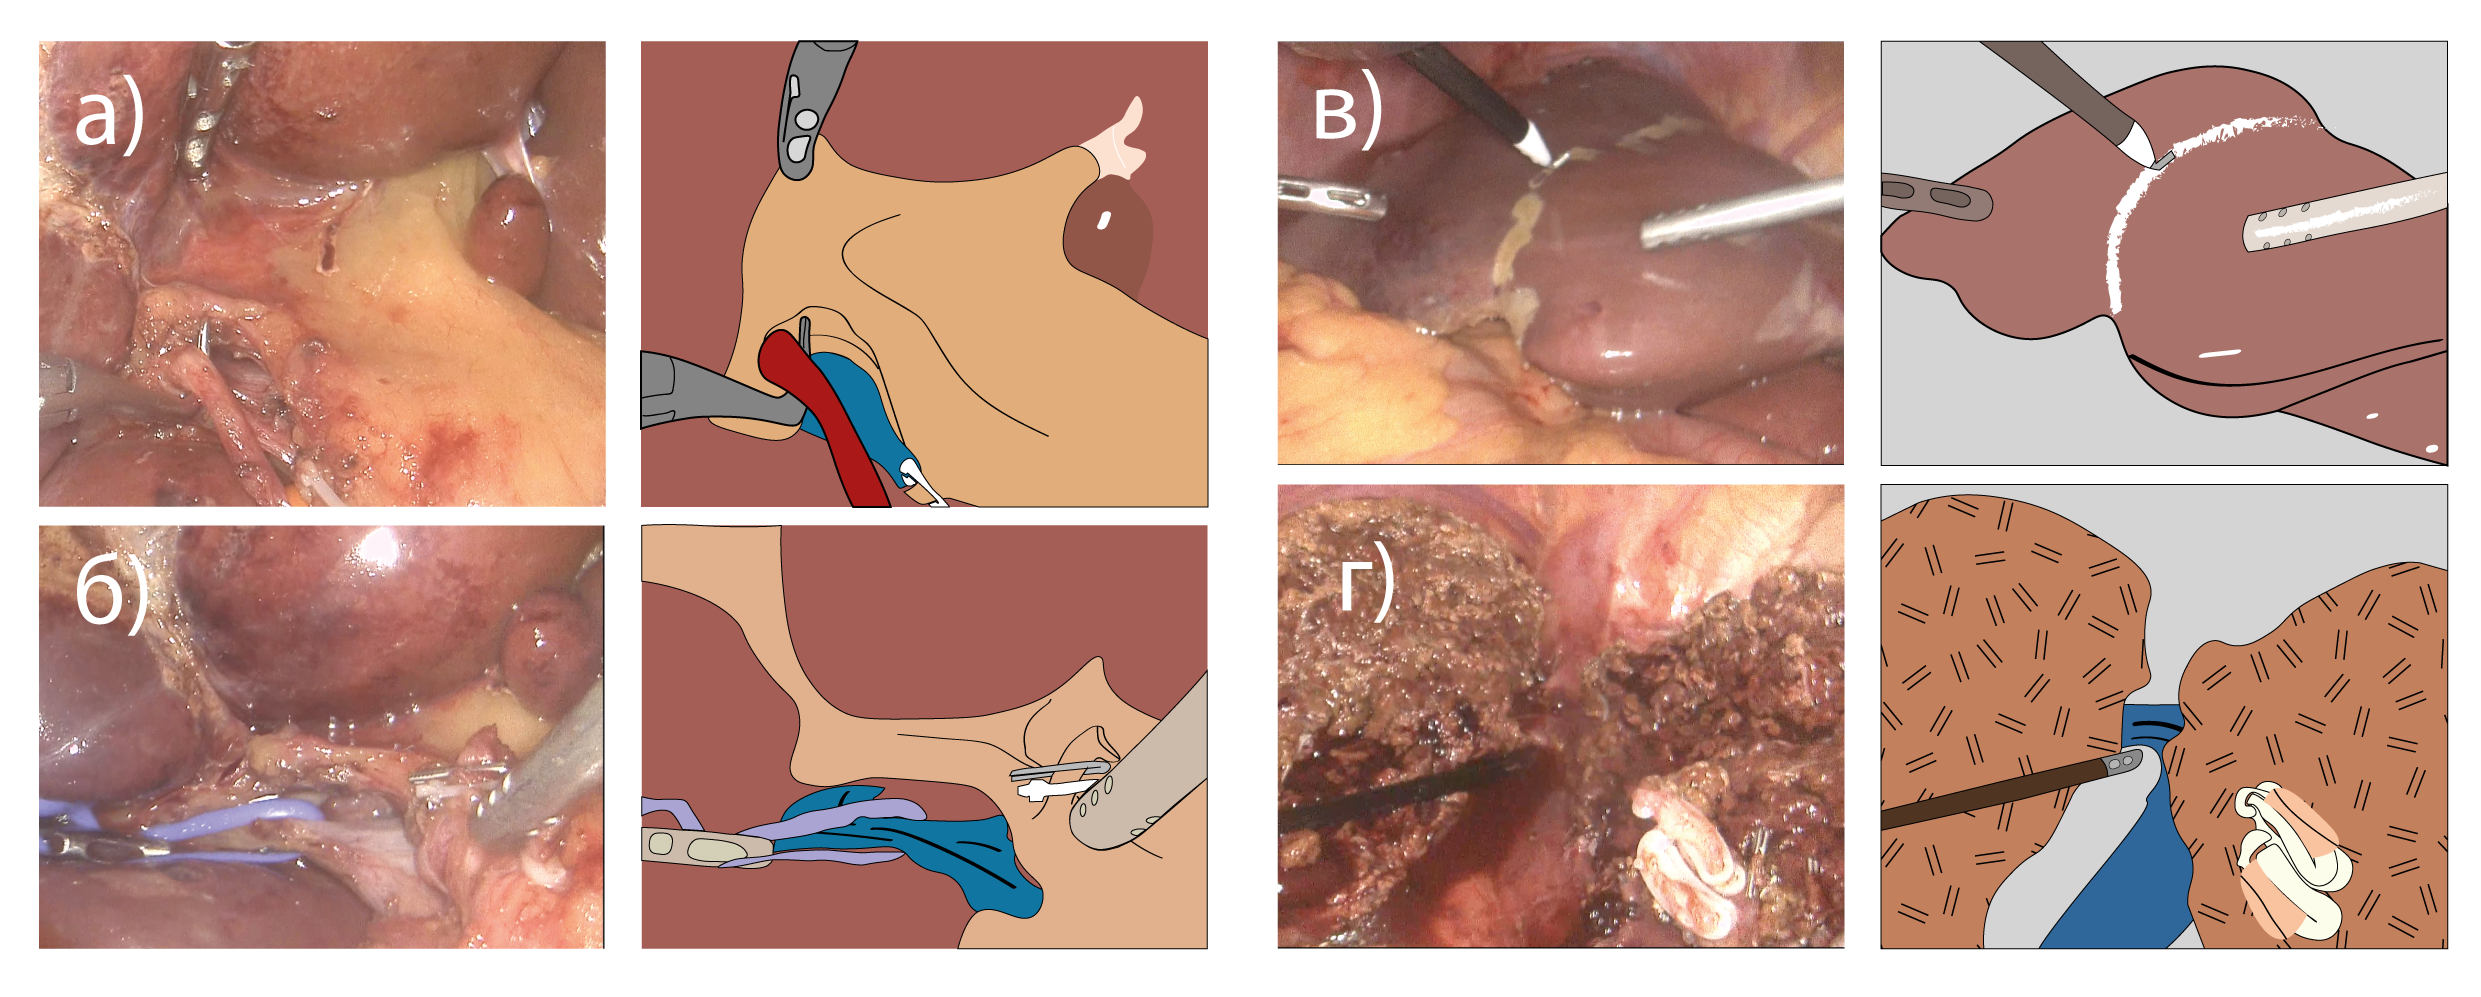
\includegraphics[width=0.9\textwidth]{Illustrations/Chapter_01/RightLobe_Horizontal.png}
\label{fig:RightLobe}

\medskip
\small
а) диссекція правої печінкової артерії, б) диссекція правої ворітної вени, в) намічення лінії транссекції паренхіми вздовж лінії Кантля, г) виконана транссекція паренхіми, виділена права печінова вена.


\end{figure}

\subsubsection{Секцієектомії та центральні резекції}

Окрім \acrshort{llhe} та \acrshort{lrhe} обширні резекції включають в себе праву передню, праву задню та ліву медіальну секцієектомії, мезогепатектомію. Технічно такі операції вважаються складнішими за класичні гемігепатектомії, так як включають дві площини резекції, що знаходяться під кутом одна до одної. Не дивлячись на це, в серії дослідженнь показано, що такі втручання є безпечними та відтворюваними в експертних центрах \cite{Honda2014, Cheng2015, Kim2017, Siddiqi2018}. 

\subsubsection{Складні локалізації}

Постерокраніальні сегменти (Sg 7,8) та каудальна лобектомія певний час вважались недоступними для лапароскопічного доступу через високе незручне розтажування обмежене ребрами та куполом діафрагми, та анатомічну близкість до печінкових вен та нижньої порожнистої вени (\acrshort{ivc}). В 2014 роци Ban D. та співавтори розробили шкалу складності для \acrshort{llr}, де віднесли ізольовані лапароскопічні резекції Sg 7 та 8 до резекцій вищого ступеню складності, порівняно з резекціями інших анатомічних ділянок. Для полегшення доступу до постерокраніальних сегментів Ikeda T. була запропонована напівпронована позиція пацієнта та латеральний доступ до Sg 7-8 \cite{Ikeda2014}.

Пізніше Honda G. та співавторами була опублікована методика анатомичної резекції Sg 7 з внутрішньопечінковим доступом до сегментарного  гліссону \cite{Okuda2017}, а Inoue Y. показано спосіб резекції Sg 6, 7 та 8 з латерального доступу з використанням трансторакальних троакарів \cite{Inoue2017}.  Такж описаний метод виконання атипових резекцій печінки трансторокальним доступом при вираженому злуковому процесі в черевній порожнині \cite{Kruger2014}. Суть методу полягає в доступі до Sg 8 з правої плевральної порожнини шляхом розсічення правого куполу діафрагми.

На теперішній момент анатомічні \acrshort{llr} Sg 7 та 8 печінки є доступними та стандартизованими втручаннями (Рис. \ref{fig:Complex_localisation_Sg7}, \ref{fig:Complex_localisation_Sg8}) 


\begin{figure}[h]
\caption{Лапароскопічна анатомічна резекція Sg 7 з приводу HCC у виконанні авторів}

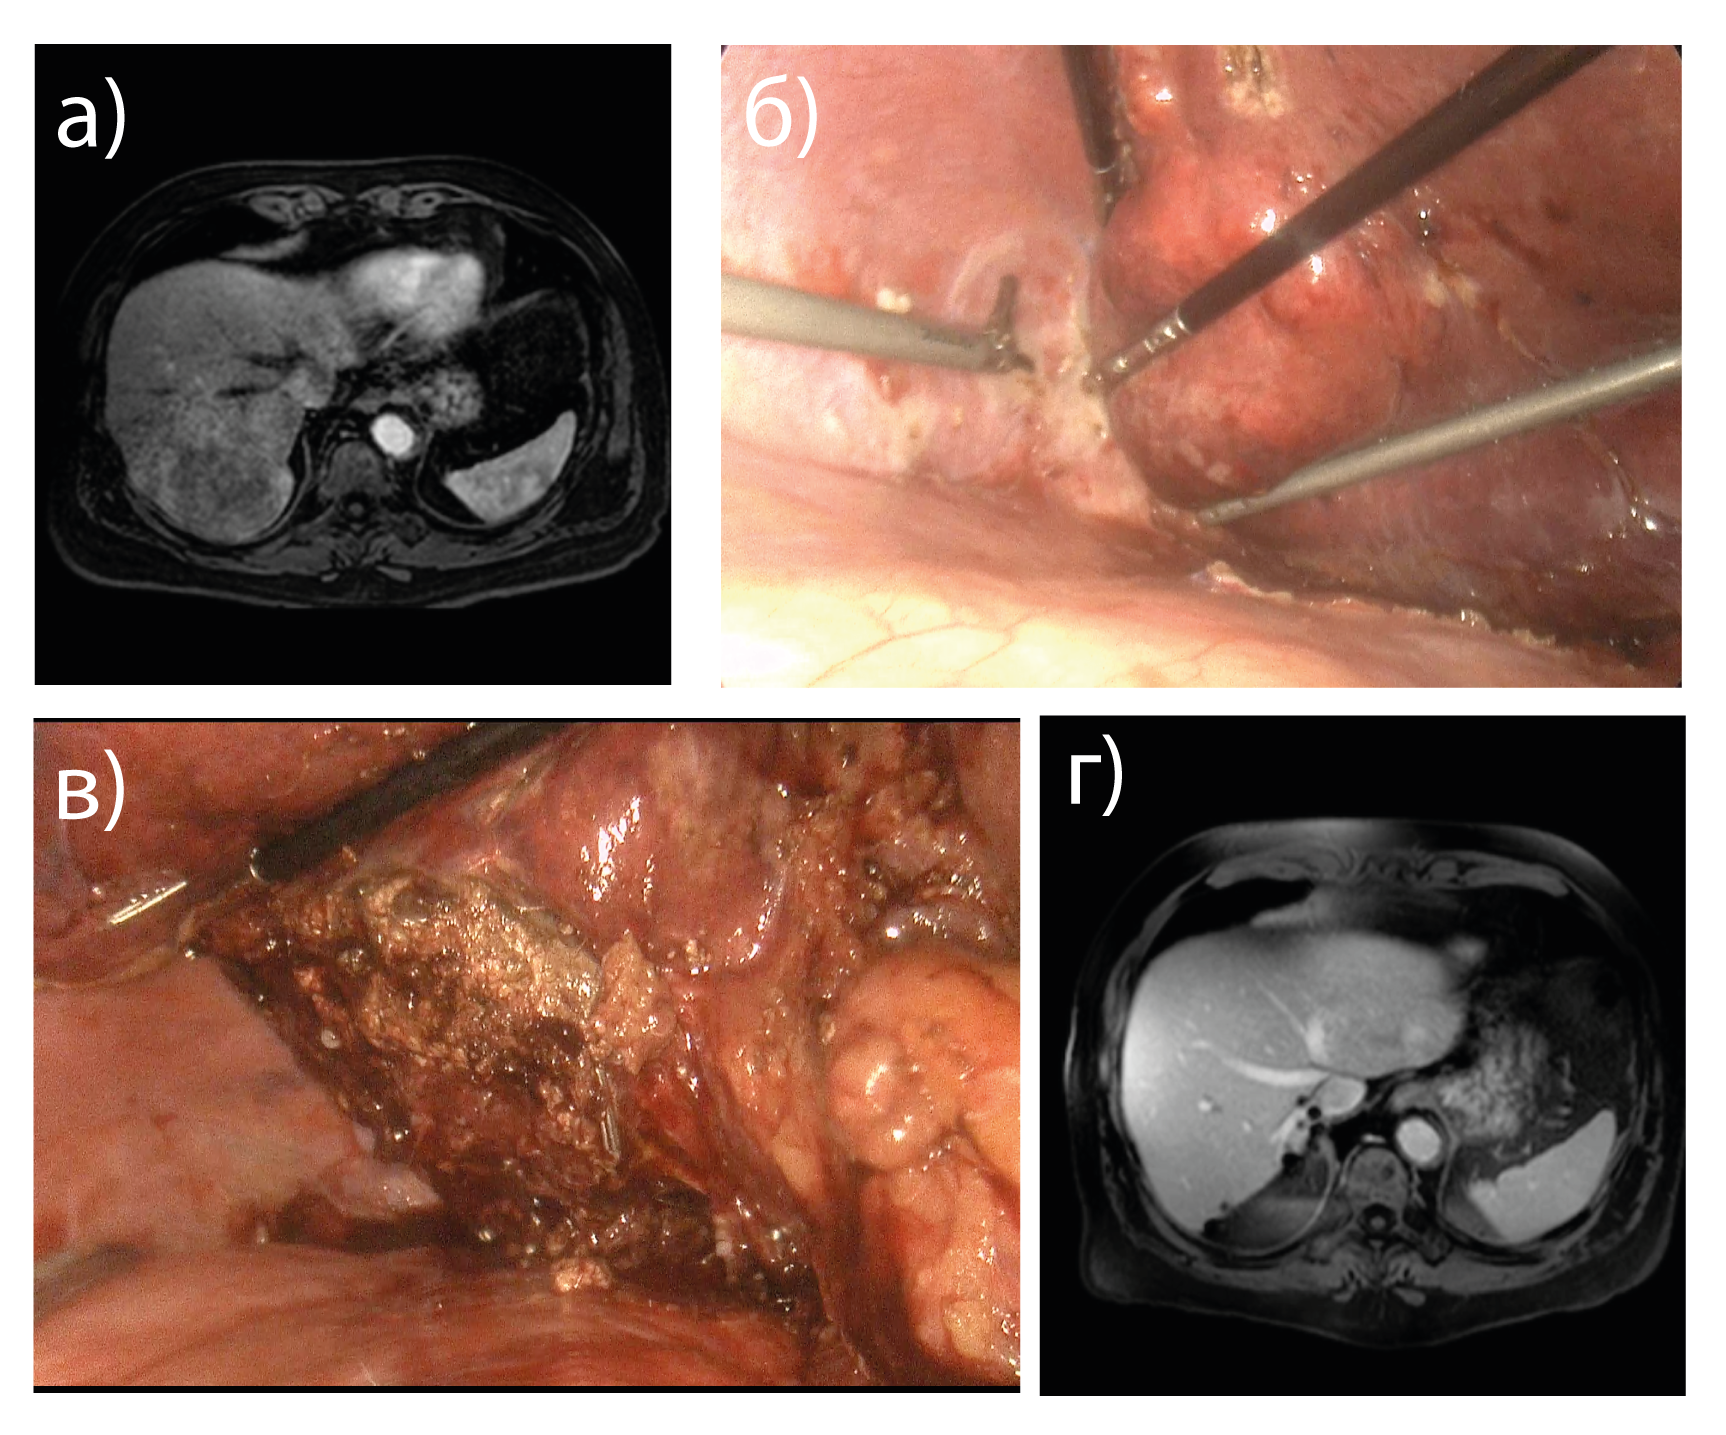
\includegraphics[width=0.9\textwidth]{Illustrations/Chapter_01/Complex_localisation_Sg7.png}
\label{fig:Complex_localisation_Sg7}

\medskip
\small
а) передопераційне \acrshort{mri} \acrshort{hcc}. Пухлина розміром 5 см. розташована в Sg 7,  б) діафрагмальна поверхня Sg 7 печінки з пухлиною, в) резекційна поверхня, г) післяопераційне \acrshort{mri} через 3 місяці після операції.

\end{figure}


\begin{figure}[h]
\caption{Лапароскопічна резекція Sg 8 з приводу ехінококозу у виконанні авторів}

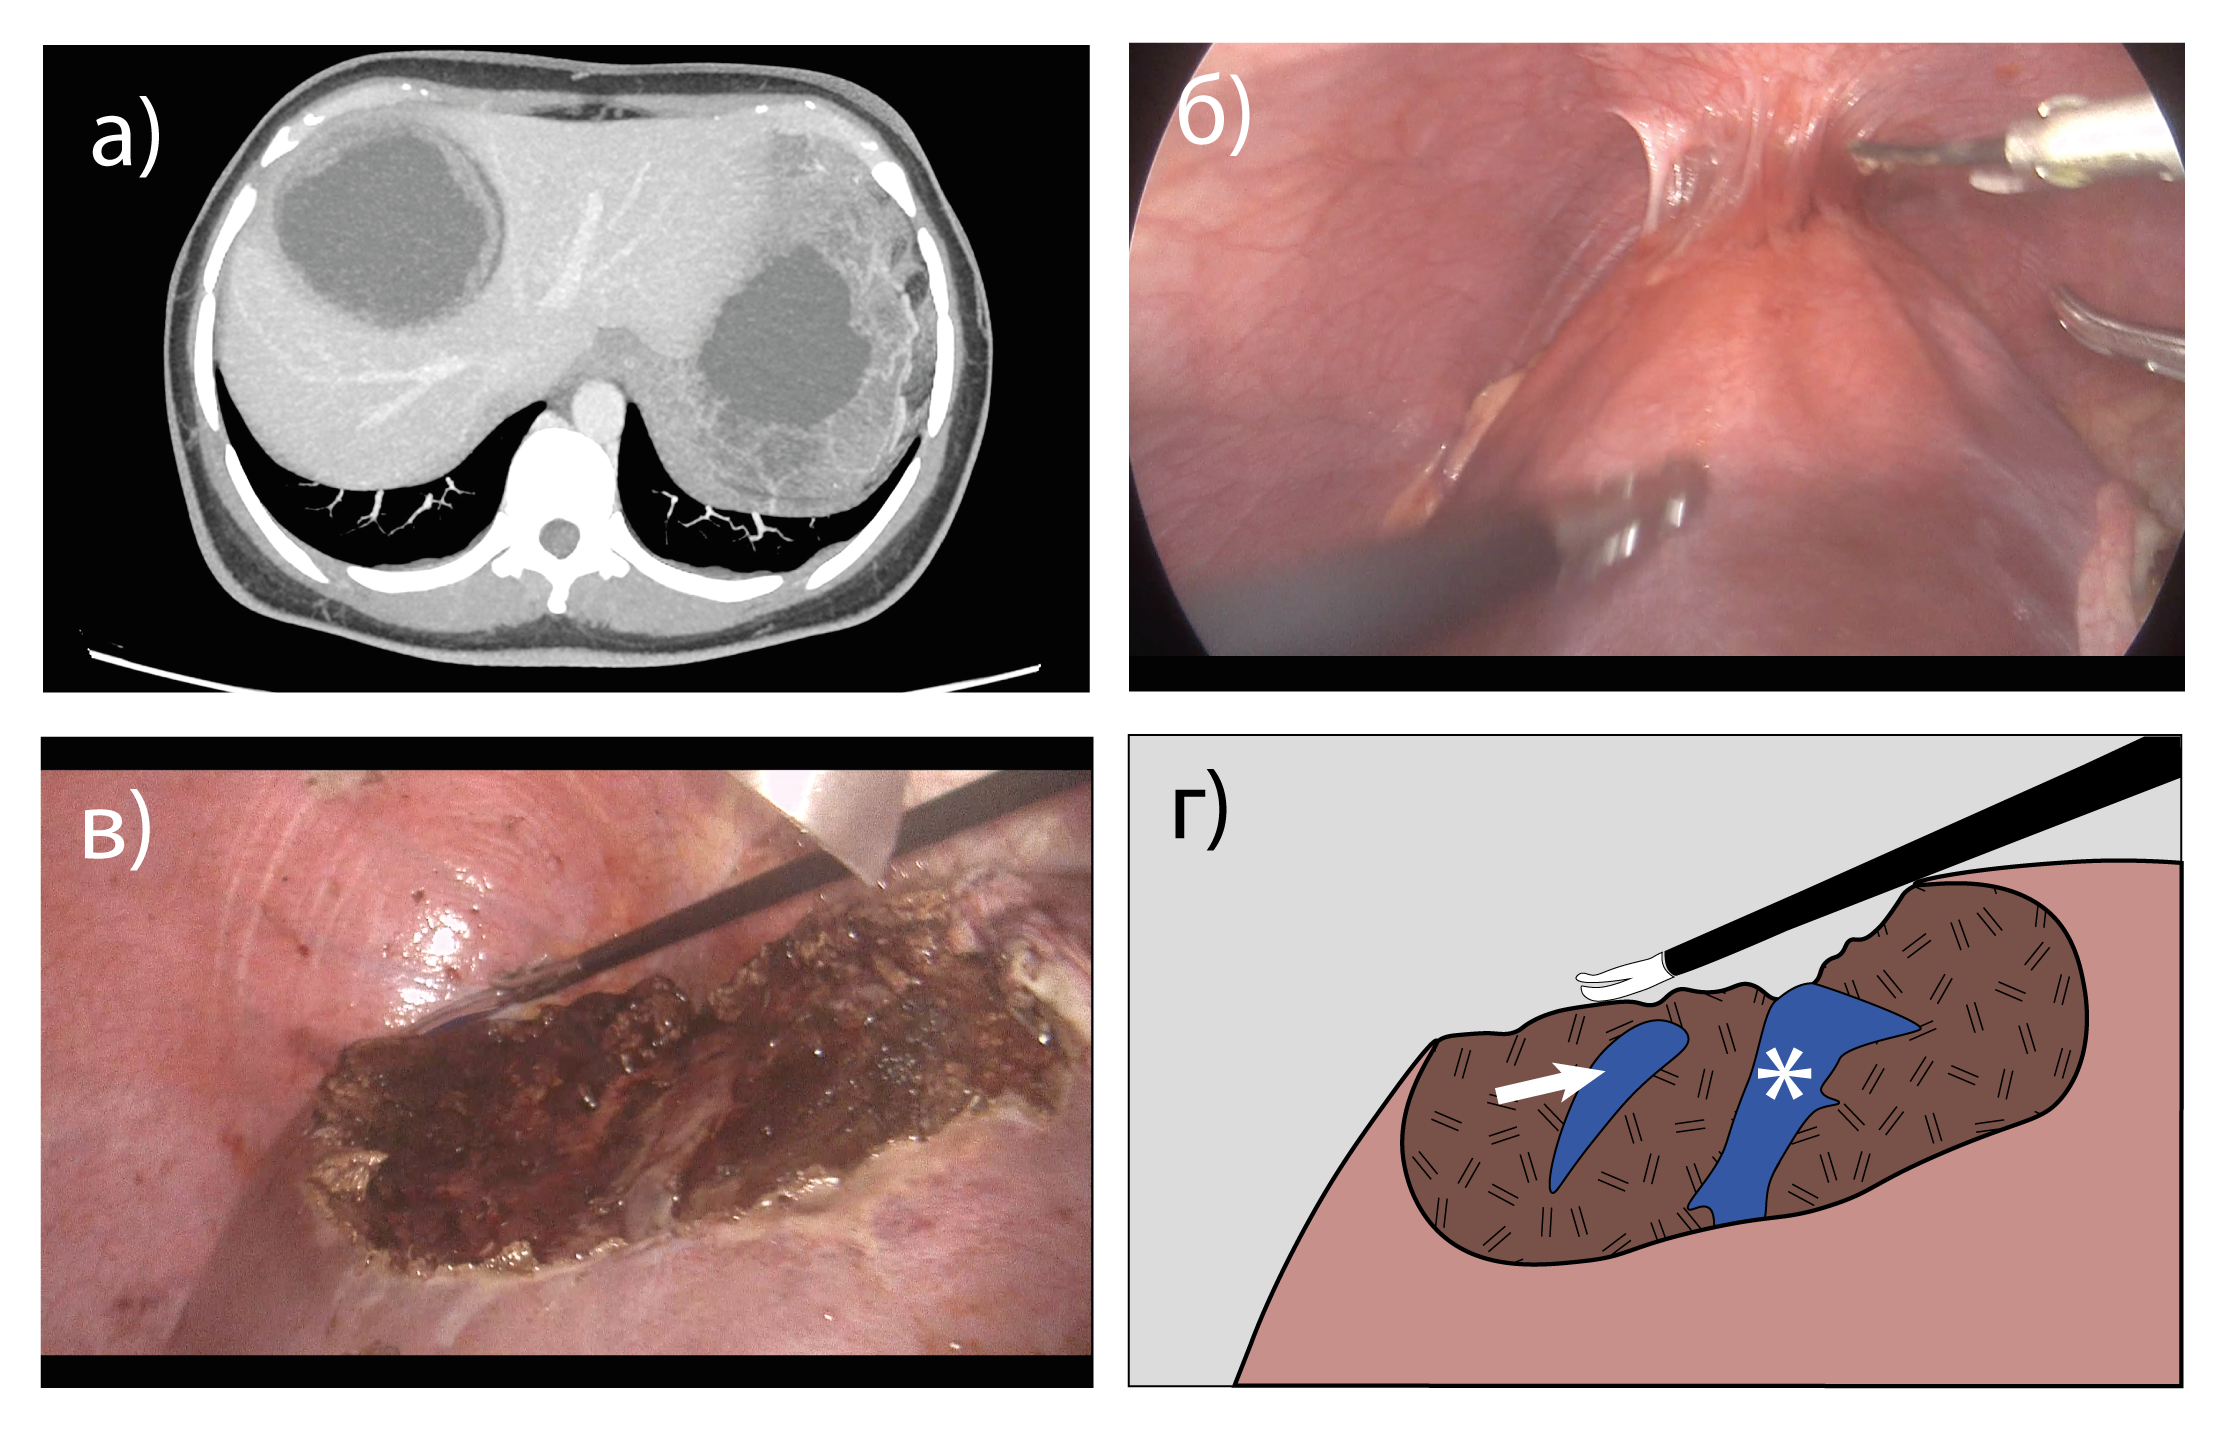
\includegraphics[width=0.9\textwidth]{Illustrations/Chapter_01/Complex_localisation_Sg8.png}
\label{fig:Complex_localisation_Sg8}

\medskip
\small
а) \acrshort{ct} ехінококової кисти, яка прилягає до  серединної печінкової вени, б) діафрагмальна поверхня Sg 8 печінки з кистою, в) резекційна поверхня, г) устя серединної та лівої печінкових вен (відмічено зірочкою) та приток правої печінкової вени (помічено стрілкою) в площині резекції.

\end{figure}





Складність каудальної лобектомії обумовлена тим, що перший сегмент розташований в позаду печінки і безпосередньо межує з \acrshort{ivc}, що робить його пряму візуалізацію неможливою та суттєво ускладнює хірургічний доступ. Окрім того каудальна доля має власні окремі печінкові вени, які дренуються в запечінковий сегмент \acrshort{ivc}, що підвищує ризик кровотечі під час його мобілізації і робить лапароскопічну каудальну лобектомію (\acrshort{lce}) складним втручанням. 
    
В літературі є обмежені згадки про досвід виконання \acrshort{lce} переважно у вигляді кейс-репортів та невеликих серій \cite{Machado2018, Cheung2016, Koh2017, Jin2018}. Найбільшою небезпекою, пов'язаною \acrshort{lce} вважають ризик розвитку масивної неконтрольованої кровотечі з передньої стінки \acrshort{ivc} або задньої стінки серединної печінкової вени (\acrshort{mhv}), при цьому загальна морбідність складає лише 6,6\% \cite{Araki2018}. Альтернативою до лапароскопічного підходу для виконання каудальної лобектомії може стати використання роботичних систем, які полегшують маніпуляції в обмеженому просторі \cite{Marino2018a}.

\subsection[Комплексні резекції]{Комплексні резекції у поєднанні з резекцією судин чи жовчних протоків, розширеною лімфодиссекцією}

У  пацієнтів з поширеними формами метастазів колоректального раку в печінку (\acrshort{crlm}), \acrshort{hcc} чи \acrshort{phcc}  може спостерігатись інвазія в магістральні структури печінки - ворітну вену, печінкові вени або жовчні протоки. Такі пацієнти потребують хірургічного лікування у вигляді резекції печінки в комбінації із судинною або біліарною резекцією. В більшості випадків необхідність комплексної резекції є показом до відкритого втручання, проте деякими авторами описана можливість виконання таких втручань в лапароскопічному варіанті. \cite{Kobayashi2015, Tardu2016, Procopio2020, Matsukuma2020}.

\subsubsection{Резекції судин}

В літературі наявні згадки про невелику кількість випадків резекцій магістральних судин виконаних під час проведення лапароскопічної резекції печінки - 3 кейс-репорти та одне дослідження серії з 6 хворих. 

Так Nomi T. та співавт. повідомляють про успішний випадок крайової резекції \acrshort{ivc} під час проведення \acrshort{lrhe} переднім доступом у 58-річного пацієнта з приводу \acrshort{crlm} \cite{Nomi2015a}. Пізніше Vega E. та співавт. виконали \acrshort{lce} з частковою резекцією \acrshort{ivc} 54-річному пацієнту, що страждав \acrshort{hcc} на фоні цирозу \cite{Vega2020}. 

Lopez-Ben та співавтори показали двохетапний лапароскопічний підхід при видаленні білобарних \acrshort{crlm} 66-річному пацієнту (Рис. \ref{fig:Vascular_resection}) . Першим етапом була виконана лапароскопічна правобічна задня секцієектомія (\acrshort{lrps}) з резекцією та реконструкцією шляхом формування судинного анастомозу правої печінкової вени (\acrshort{rhv}). Під час другого етапу була виконана \acrshort{llhe}. Автори повідомляють про хороший онкологічний ефект операції та відсутність рецидивів під час огляду через 2 роки після втручання \cite{Lopez-Ben2020}.

\begin{figure}[!ht]
\caption{Лапароскопічна правобічна секцієектомія як перший етап двоетапної резекції з приводу \acrshort{crlm} у виконанні Lopez-Ben \cite{Lopez-Ben2020}}

\includegraphics[width=0.95\textwidth]{Illustrations/Chapter_01/Vascular_resection.png}
\label{fig:Vascular_resection}

\medskip
\small
а) \acrshort{ct} \acrshort{crlm}, який прилягає до правої печінкової вени, б) лінія демаркації після перетискання глісону правої задньої секції печінки, в,г) інвазія метастазу в праву печінкову вену (пухлина помічена зірочкою, вена відмічена на схемі синім кольором), ґ, д) резекція стовбура правої печінкової вени, е) реконструкція правої печінкової вени анастомозом кінець в кінець, є) фінальний вигляд вени після накладання анастомозу (лінія анастомозу відмічена пунктиром)

\end{figure}
	
Єдине дослідження серії випадків судинних резекцій під час проведення \acrshort{llr} належить Morise Z. та співавторам \cite{Morise2015a}. Автори заявляють про досвід 98 \acrshort{llr} з приводу \acrshort{hcc} на фоні цирозу, 6 з яких було виконано резекцію стовбура однієї з магістральних печінкових вен за допомогою лінійного степлера.

Не дивлячись на достатньо поширене застосування резекції та реконструкції стовбура ворітної вени під час виконання лапароскопічної панкреатодуоденальної резекції \cite{Kendrick2011, Garbarino2018, Wei2019} нами не було знайдено джерел, що описують застосування портопластики під час проведення \acrshort{llr}, що скоріше за все пов'язано із її технічною складністю та обмеженістю показів. 

\subsubsection{Біліарні реконструкції}

В лапароскопічному варіанті, як самостійне втручання гепатикоєюностомія широко використовується при кистах та стриктурах холедоха, як паліативне втручання, а також як частина панкреатодуоденальної резекції при пухлинах голівки підшлункової залози. Резекція позапечінкових жовчних шляхів є обов'язковим етапом радикальних резекцій печінки з приводу \acrshort{phcc} а також може бути застосована при пухлинній інвазії іншими пухлинами. Згідно доступних даних \acrshort{llr} з приводу  \acrshort{phcc} все ще є новітньою процедурою на стадії вивчення, тому досвід виконання таких операцій обмежений кейс-репортами \cite{Lin2014, Machado2014} або невеликими серіями \cite{Ratti2020}. Таким чином в експертних центрах гепатикоєюностомія є технічно доступним етапом при виконанні \acrshort{llr}, а впровадження роботичної хірургії дає надію на її більш широке застосування \cite{Machado2019, Giulianotti2010}

\subsubsection{Розширена лімфаденектомія}

Лімфодиссекція є стандартизованим етапом багатьох лапароскопічних операцій з приводу онкопатології, зокрема в мініінвазивній гінекології та хірургії шлунково-кишкового тракту \cite{Eshuis2018, Jung2019}. В резекційній хірургії печінки лімфодиссекція показана при наявності локального позапечінкового ураження лімфовузлів наприклад при \acrshort{crlm}. Не дивлячись на те, що  онкологічна ефективність привентивної лімфаденектомії при \acrshort{llr} з приводу \acrshort{ihcc} остаточно не доведена \cite{Weber2015, Zhou2019a}, багато хірургів рекомендують її рутинне виконання з метою адекватного стадіювання пухлини та визначення прогнозу \cite{Waisberg2018, Ratti2020a}.

Більшість данних про лімфаденектомію як етап \acrshort{llr} представлені у вигляді кейс-репортів та серій випадків. Їх узагальнення  наведено Levi Sandri G.B. та співавторами в оглядовій статті, на основі чого автори роблять висновок про безпечність та доступність лапароскопічного підходу \cite{Colasanti2017}. 

Також є результати моноцентрового псевдорандомізованого дослідження в якому Ratti F. зі співавторами порівнюють 20 пацієнтів, що перенесли \acrshort{llr} з приводу \acrshort{ihcc} із 60 аналогічними відкритими операціями. За отриманими результатами \acrshort{llr}, серед яких 85\% великих резекцій, були не гіршими від відкритих втручаннь за показниками морбідності та безрецидивної виживаності, а також були асоційовані із меншою крововтратою та більшою кількістю видалених лімфовузлів \cite{Ratti2016a}. 

\subsection{Технологія ALPPS} 

В перше технологія Associating Liver Partition and Portal vein Ligation for Staged hepatectomy(\acrshort{alpps}) була запропонована в 2011  Lang H.  \cite{Baumgart2011} в якості альтернативи звичайній двоетапній резекції печінки з лігуванням ворітної вени. Суть нововведення полягала в тому, що на першому етапі проводять санацію планованого печінкового залишку, лігування ворітного притоку  частини печінки, що видаляють та транссекція паренхіми. При цьому за рахунок потужного викиду прозапальних факторів протягом 7-14 днів відбувається швидкий приріст об'єму планованого печінкового залишку, після чого виконують другий етап, під час якого видаляють депорталізовану на першому етапі частину печінки. 

Методика привернула увагу та отримала багатьох прихильників серед гепатобіліарних хірургів, як метод, що дозволяє значно розширити межі резектабельності у пацієнтів з обширним пухлинним ураженням. Критики цієї методики зазначають, що вона має високу частоту післяопераційних ускладненнь та ризики прогрессії пухлини між першим та другим етапами. 

Для подолання цих недоліків Brustia R. та співавторами було запропоновано виконувати втручання в лапароскопічному варіанті \cite{Brustia2013}. Наразі загальна кількість таких операцій не велика, що може бути пов'язано з тим, що відкрита  \acrshort{alpps} є відносно новим та методом, який досі знаходиться на етапі дослідження \cite{Melandro2019}.

Так, Michal K. та співавтори \cite{Michal2020} за результатами метааналізу 23 джерел порівняли 46 мініінвазивних та 1088 відкритих \acrshort{alpps}, та дійшли до висновку, що лапароскопічні та роботичні втручання дозволяють знизити частоту ускладненнь порівняно з відкритими втручаннями та отримати більший ступінь гіпертрофії порівняно з емболізацією ворітної вени. 

\subsection{Лапароскопічна донорська резекція печінки} 

Трансплантація печінки від живого донора стала радикальним методом лікування дифузних захворюваннь та деяких пухлин печінки в умовах відсутності або обмеженої кількості трупних донорів. На відміну від резекцій з приводу новоутвореннь, під час виконання донорської резекції печінки перед хірургом стоять два завдання -  забезпечення безпеки та збереження здоров'я донора та забір реплантабельного та функціонального трансплантату з достатньою довжиною та придатним для пластики краєм ворітної та печінкових вен, печінкової артерії та жовчних протоків. 

Для зменшення ризику ускладненнь та раннього повернення працездатності донору в 2002 р. Cherqui D. та співавторами було запропоновано виконання донорського забору лівої латеральної секції в лапароскопічному варіанті при трансплантації дітям \cite{Cherqui2002a}. Пізніше техніка операції була адаптована та імплементована деякими центрами. Так наприклад Kim K-H. та свпіватори повідомляють про переваги лапароскопічного донорського забору лівої латеральної секції у вигляді зменшення терміну госпіталізації та пришвидшення реабілітації донора за результатами порівняння 11 таких втручаннь із 11 відкритими донорськими резекціями \cite{Kim2011}. 

Технічно більш складна донорська правобічна гемігепатектомія певний час залишалась недоступною для чисто лапароскопічного доступу. Запропоновані \acrshort{hals} та \acrshort{hlr} підходи не набули широкого розповсюдження \cite{Koffron2006, Thenappan2011, Lin2013}. Лише в 2013 р. Soubrane O. та співавторами була показана можливість донорського забору трансплантату правої долі печінки в чисто лапаропскопічному доступі \cite{Soubrane2013}. 

На теперішній момент лапароскопічний донорська гепатектомія активно застосовується більшістю великих спеціалізованих трансплантаційних центрів. Доступні результати псевдорандомізованих порівняльних дослідженнь, які демонструють переваги лапароскопічних донорських заборів над відкритими \cite{Broering2018, Park2019a}. Також показано безпеку лапароскопічного забору для реципієтнів \cite{Kwon2018a}. Йде дискуссія про стандартизацію та повсюдне впровадження методу \cite{Au2018, Samstein2018}

Таким чином за свою майже 30-річну історію \acrshort{llr} вийшла далеко за межі крайових та атипових резекцій антеролатеральних сегментів та впевнено конкурує з відкритими втручаннями у всіх галузях гепатобіліарної хірургії. 

\section{Покази до виконання лапароскопічних резекцій печінки}

Технічні можливості лапароскопічної хірургії постійно зростають а хірургічна техніка вдосконалюється завдяки чому більшість втручаннь, що раніше виконувались лише у відкритому доступі зараз можлива і в лапароскопічному варіанті. Враховуючи сучасні досягнення покази до \acrshort{llr} практично не відрізняються від показів до \acrshort{olr} - лапароскопічний досуп не обмежує хірургічні можливості, проте додає певні, властиві саме йому, особливості. 

Серед показів до резекції печінки розрізняють злоякісну та доброякісну патологію. Серед онкопатології, на долю якої приходиться 60-80\% резекцій  найбільш частими показами до хірургічного лікування є первинні пухлини печінки та жовчних шляхів, а саме гепатоцелюлярна карцинома (\acrshort{hcc}), внутрішньопечінкова (або масформуюча) холангіокарцинома (\acrshort{ihcc}), перихіларна холангіокарцинома (\acrshort{phcc}), рак жовчного міхура (\acrshort{gbc}) та метастази колоректального раку в печінку \acrshort{crlm}. 
В цьому розділі ми зосередимось на тих видах хірургічної патології печінки, при яких застосування мініінвазивного підходу дає можливість отримати позитивні результати. 

\subsection{Гепатоцеллюларна карцинома}.
Гепатоцеллюлярна карцинома (\acrshort{hcc}) є п'ятою за частотою серед причин летальності від онкологічних захворюваннь. Причиною цього є  виявлення пізніх стадій захворювання через його асимптоматичний перебіг. Поширені форми \acrshort{hcc} характеризуються судинною інвазією, яка значно утруднює їх хірургічне лікування, а також наявністю у більшості хворих супутнього хронічного захворювання печінки та цирозу які суттєво погіршують печінкову функцію. Окрім того \acrshort{hcc} є хіміорезистентною пухлиною, що робить системну хіміотерапію не ефективною.

Сучасний підхід до лікування \acrshort{hcc} базується на виборі методу лікування в залежності від стадії пухлини. Найбільш часто вживаною системою стаціювання \acrshort{hcc} є барселонська (\acrfull{bclc}, \acrshort{bclc}) \cite{Llovet2003}. Згідно \acrshort{bclc} хірургічне лікування показано на ранній та дуже ранній стадіях \acrshort{hcc}, коли пухлина представлена солітарними резектабельними вузлами, а можливми опціями лікування є етанолова або радіочастотна абляція, відкрита або лапароскопічна резекція та трансплантація печінки. 

При дуже ранній стадії \acrshort{hcc} за \acrshort{bclc} з розміром вогнища до 2 см найбільш ефективні етанолова та радіочастотна абляція  \cite{Cucchetti2013}. Пацієнтам з \acrshort{hcc} в межах міланських критеріїв та декомпенсованим цирозом печінки оптимальним методом лікування є трансплантація печінки \cite{Colombo2016}. Для всіх інших пацієнтів з резектабельними формами \acrshort{hcc} методом першого вибору є резекція печінки \cite{Heimbach2018, Kudo2011}. 

\subsubsection{Анатомічні та неанатомічні резекціії з приводу \acrshort{hcc}}

\acrshort{hcc} --- агресивна високоінвазивна пухлина, яка має тенденцію до ураження малих та великих внутрішньопечінкових судин, периваскулярних компартментів та жовчних шляхів. Портальні тромби спричинені судинною інвазією можуть викликати кавернозну трансформацію та перивенозну колатеральну сітку. Мікросудинна інвазія це типова особливість \acrshort{hcc}, характерна переважно менш діфференційованим пухлинам, яка підтверджує агрессивну біологію пухлини. Незалежними предикторами мікроваскулярної інвазії є розмір пухлини більший 5 см., та менший ступінь дифференціації \cite{Zimmermann2017}. Інвазія в дрібні внутрішньопечінкові гілки ворітної вени може приводити до локального ретропортального кровотоку та периферійного внутрішньопечінкового розповсюдження у вигляді числених метастатичних вузлів по ходу судин в межах портального судинного басейну локальної анатомічної ділянки (Рис. \ref{fig:HCC_vascular_invasion}). 


\begin{figure}[h]
\caption{Механізм виникнення пухлинного портального тромбозу при ГЦК}
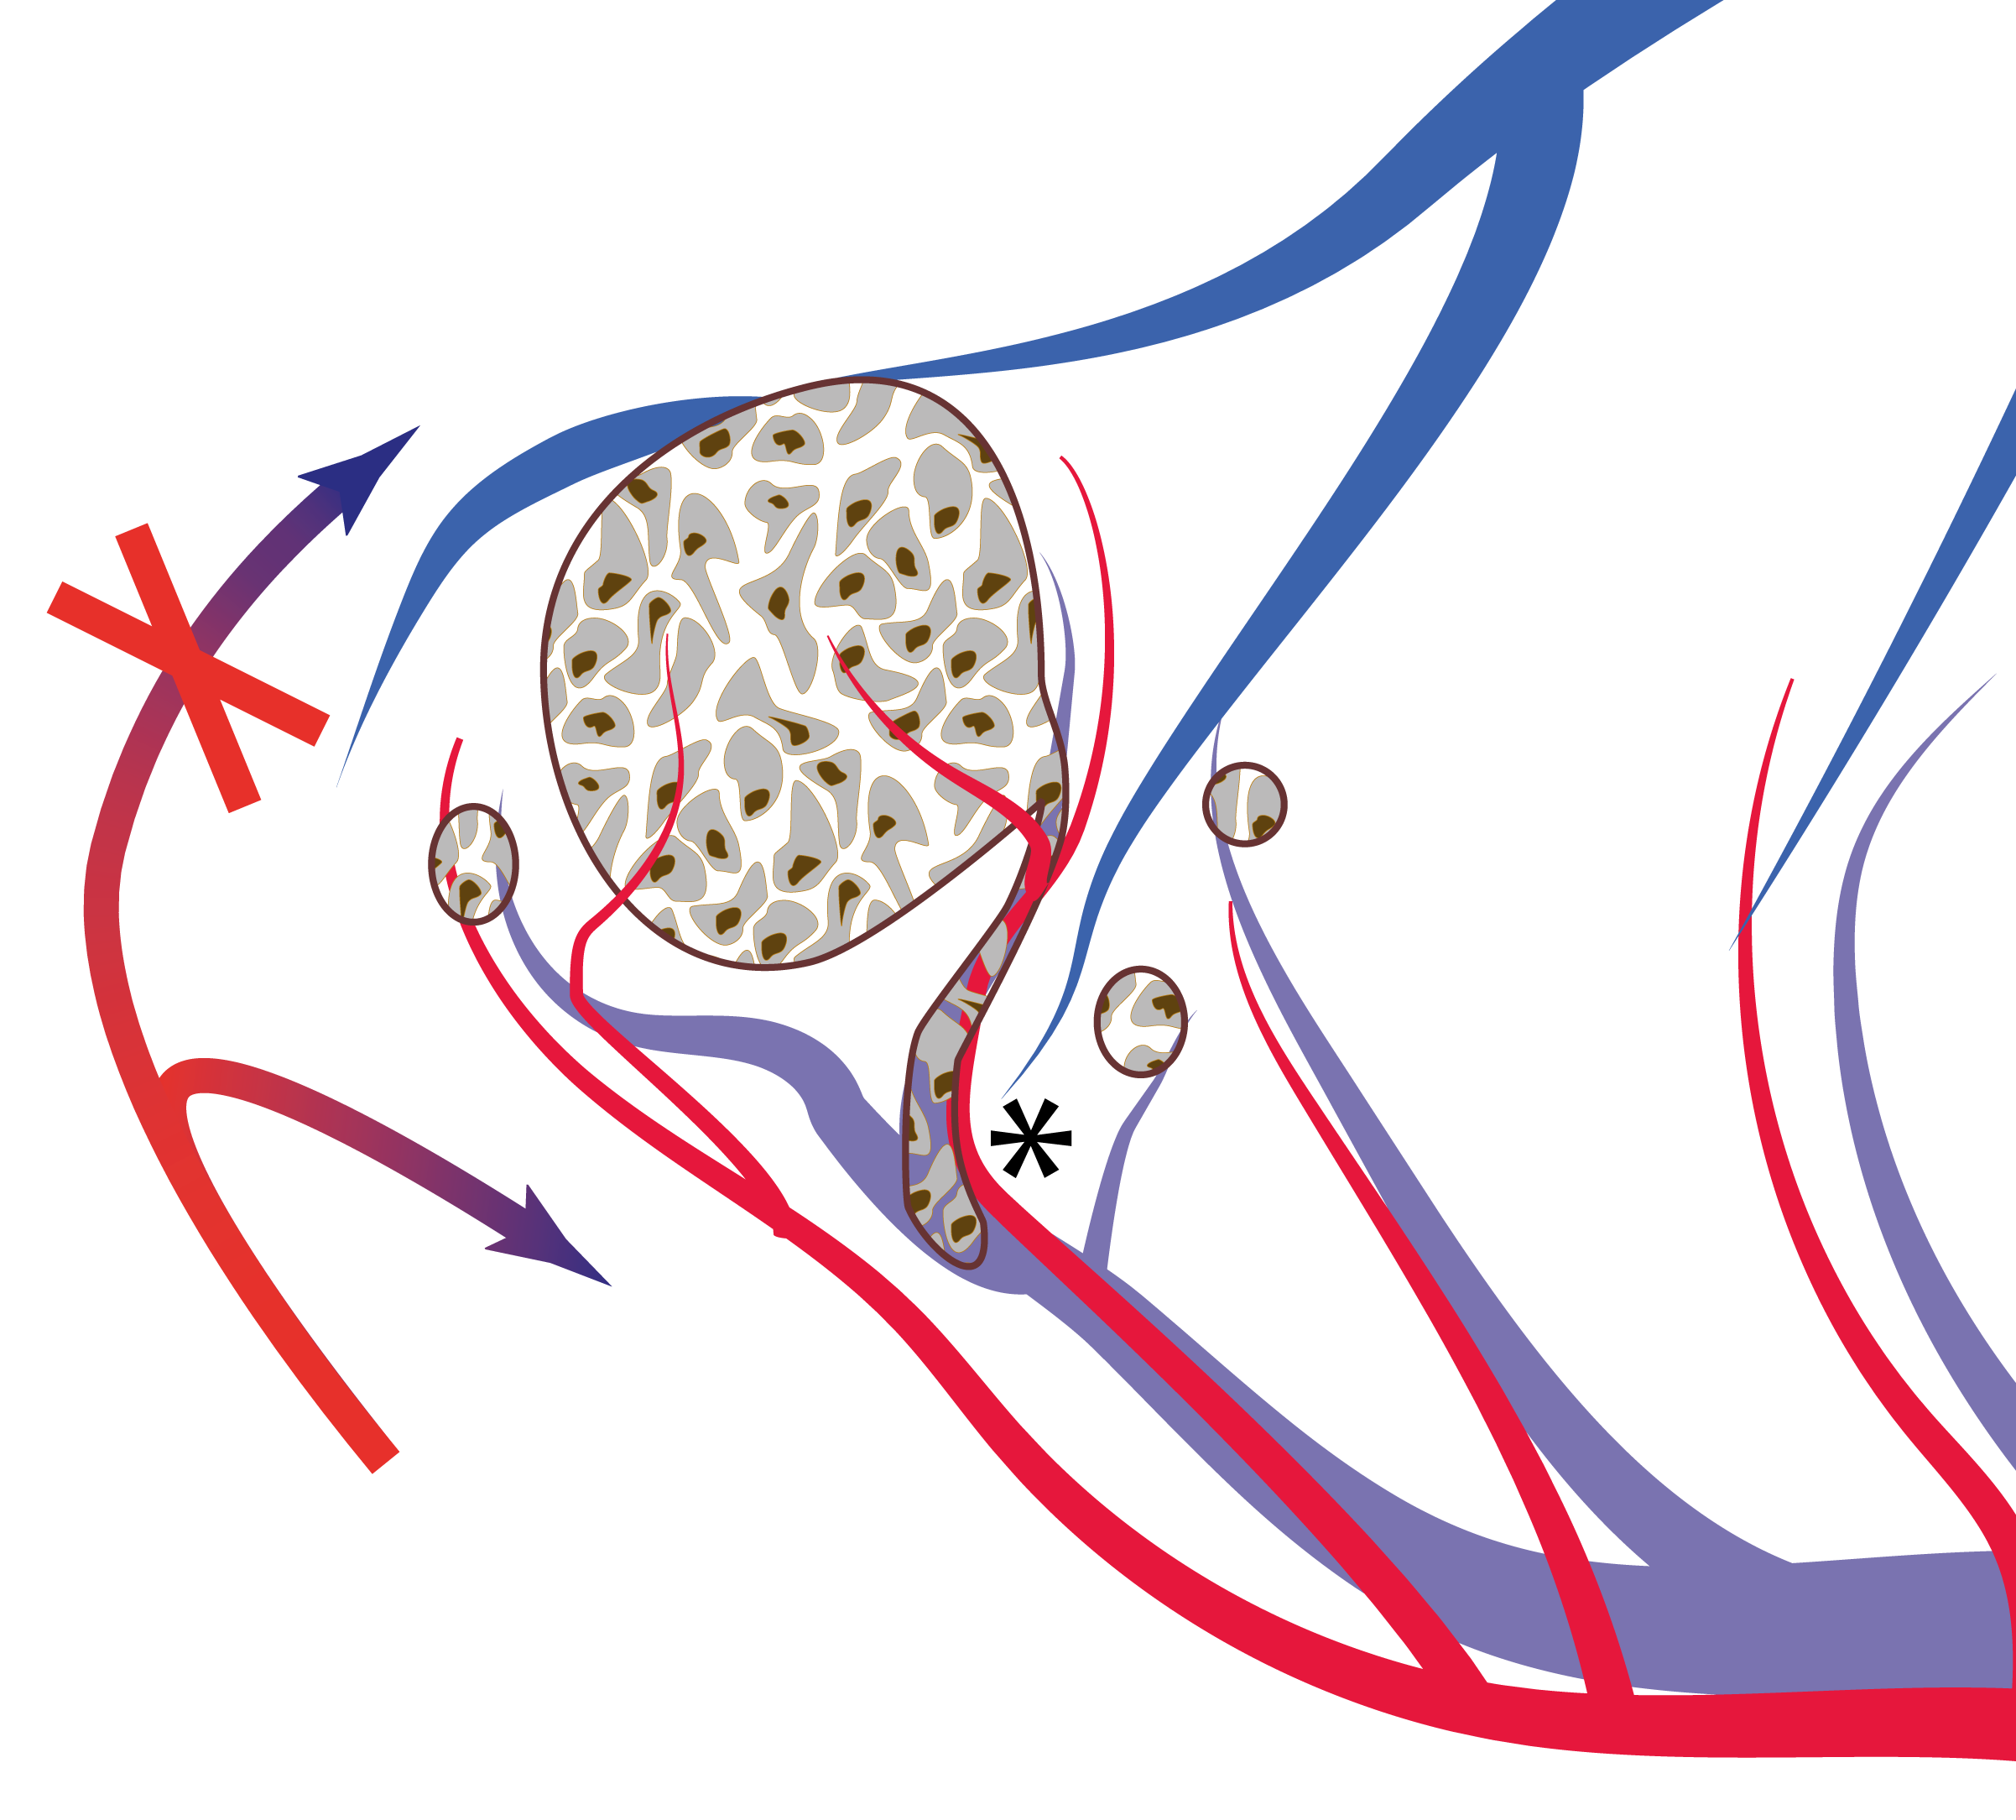
\includegraphics[width=0.9\textwidth]{Illustrations/Chapter_01/HCC_vascular_invasion.png}
\label{fig:HCC_vascular_invasion}

\medskip
\small
Під час свого росту пухлина інвазує дрібні гілки печінкових вен та створює локальну венозну гіпертерзію. Це призводить до локального реверсу кровотоку (помічено стрілками) в портальних гілках та росту пухлинного тромбу (помічено зірочкою) проти напрямку портального кровотоку.

\end{figure}




Враховуючи схильність \acrshort{hcc} до локального метастазування в межах анатомічних ділянок методом вибору хірургічного лікування є анатомічна резекція печінки (\acrshort{alr}). На відміну від неанатомічної резекції печінки (\acrshort{non-alr}) \acrshort{alr} включає в себе ідентифікацію судинного бассейну анатомічної ділянки, що містить пухлину та видалення всієї її паренхіми. Онкологічні переваги \acrshort{alr} підтверждують більшість дослідженнь, так Makuuchi M. та співавтори \cite{Shindoh2016} в дослідженні 209 пацієнтів з цирозом класу А за Чайлдом та \acrshort{hcc} розміром $\leq$ 5 см, що були резектабельні як за допомогою \acrshort{alr} так і \acrshort{non-alr} показали перевагу \acrshort{alr} завдяки меншому ризику локальних рецидивів та більшій тривалості життя. Автори метааналізу \cite{Moris2018} 43 досліджень стверджують, що у 6839 пацієнтів яким була виконана \acrshort{alr} в порівнянні з 5590 пацієнтами з \acrshort{non-alr} були кращі загальна та безрецидивна виживаність та морбідність та рання післяопераційна летальність.

До переваг \acrshort{alr} відносять кращий онкологічний ефект, а до недоліків - вищий порівняно з \acrshort{non-alr} ризик післяопераційного порушення печінкової функції, пов'язаний з більшим об'ємом резекції, що особливо важливо для пацієнтів із цирозом печінки. Враховуючи це необхідний ретельний відбір пацієнтів для резекції печінки з приводу \acrshort{hcc}, що базується на оцінці рівню печінкової недостатності, ступеню портальної гіпертензії та загального статусу пацієнта. Американські клінічні настанови National Comprehensive Cancer Network (\acrshort{NCCN}) в якості кандидатів для резекції печінки пропонують пацієнтів з компенсованою печінковою функцією, солітарним вогнищем без макросудинної інвазії та майбутнім печінковим залишком (\acrshort{flr}) $\geq$ 20\% для здорової паренхіми та $\geq$ 30-40\% з адекватним кровопостачанням та жовчевідтоком. В клінічних настановах Європейської ассоціації вивчення хвороб печінки по лікуванню \acrshort{hcc} \cite{Galle2018a} для пацієнтів з цирозом печінки запропоновано спрощений алгорим визначення ризику \acrshort{alr}, що базується на об'ємі резекції, супеню портальної гіпертензії та печінкової недостатності. 


\begin{figure}[h]
\caption{Анатомічна резекція Sg 5 печінки з приводу \acrshort{hcc} у виконанні авторів}

\includegraphics[width=0.9\textwidth]{Illustrations/Chapter_01/HCC-Sg5.png}
\label{fig:HCC-Sg5}

\medskip
\small
а) Передопераційні \acrshort{mri} та \acrshort{ct}. Пухлина локалізована в Sg 5 печінки б) Діафрагмальна поверхня Sg 5 печінки з пухлиною  в) Транссекція паренхіми г) Резекційна поверхня ґ, д) Макропрепарат (зірочкою помічено приток від Sg 5 до правої печінкової вени, стрілками - культі сегментарних глісонів)

\end{figure}



\subsubsection{Вибір між лапароскопічною та відкритою резекцією печінки при \acrshort{hcc}} 
Окрім віддалених результатів на ефективність лікування впливає післяопераційна морбідність. Першим з двох основних факторів, які впливають на післяопераційні результати під час резекції печінки з приводу \acrshort{hcc} є крововтрата. Вищий об'єм крововтрати та замісної трансфузії препаратів крові асоційований з вищою з частотою післяопераційних ускладненнь та меншою віддаленою виживаністю \cite{DeBoer2007, Romano2012}. Крововтрата викликає імунодепрессію що сприяє розвитку хірургічних інфекцій, сепсису і збільшення ризику рецидиву в подальшому. Другим фактором є післяопераційна асцитопродукція у пацієнтів з цирозом печінки, яка є грізним ускладненням, що може призводити до великих втрат білка та рідини (до 5 літрів на добу), нагноєння післяопераційної рани та погіршання печінкової функції \cite{Ishii2014}. Окрім збільшення резистивності портального русла через його зменшення внаслідок резекції печінки та набряку печінкового залишку, механізм виникнення асцитопродукції пов'язують з декомпенсацією портальної гіпертензії внаслідок переривання портосистемної колатералізації під час лапаротомії \cite{Kanazawa2013}. 

Згідно існуючих даних, лапароскопічний підхід ефективно знижує ризики обох цих ускладненнь. За рахунок більш прецизійної техніки та позитивного тиску карбоксиперитонеуму \acrshort{llr} асоційовані з меншою інтраопераційною крововтратою, а збереження цілісності колатералей передньої черевної стінки дозволяє знизити частоту та інтенсивність післяопераційної асцитопродукції \cite{Truant2011}. Також \acrshort{llr} зменшують і загальну післяопераційну морбідніть у пацієнтів з \acrshort{hcc} на фоні цирозу при вираженій портальній гіпертензії та тромбоцитопенії < 100,000/мл про що свідчать результати міжнародного мультицентрового порівняльного псевдорандомізованого дослідження результатів лікування 1974 пацієнтів \cite{Ruzzenente2020}.

\emph{Враховуючи наведене вище оптимальними показами до \acrshort{llr} при \acrshort{hcc} є резектабельні форми пухлини всіх локалізацій без ураження магістральних судин або жовчних протоків на фоні здорової паренхіми або компенсованого цирозу печінки при відсутності показів до трансплантації печінки.}

\subsection{Рак біліарного тракту}

Рак біліарного тракту (\acrshort{btc}) - гетерогенна група захворюваннь до якої відносять внутрішньопечінкову (або масформуючу) холангіокарциному (\acrshort{ihcc}), перихіларну холангіокарциному (\acrshort{phcc}), рак жовчного міхура (\acrshort{gbc}) покази до лікування яких за допомогою \acrshort{llr} будуть розглянуті нижче, та рак дистального відділу холедоха і ампулярний рак, які не відносяться до теми цієї книги. 

\subsubsection{Внутрішньопечінкова масформуюча холангіокарцинома}

\acrshort{ihcc} є другою за частотою формою первинного рака печінки з високим потенціалом диссемінації та рецидивів, що походить із клітин проксимальних гілок жовчних протоків, на долю якої припадає до 40\% первинних пухлин печінки. Резекція печінки (Рис. \ref{fig:IHCC}) є єдиним потенційно радикальним методом та застосовується в якості першого етапу лікування \acrshort{ihcc}. Медіана виживаності пацієнтів після радикальної резекції складає 27 - 36 міс \cite{Buettner2017}. Не дивлячись на те, що вплив лімфаденектомії на виживаність при \acrshort{ihcc} остаточно не доказано рекомнедується її рутинне виконання з метою стадіювання процесу та вибору подальшого лікування. При досягненні R0 резекцийного краю необхідна системна адьювантна хіміотерапія, яка може бути доповнена хеморадіаційними методами в разі R1 резекції або позитивних лімфовузлів. При досягненні R2 резекцийного краю із макроскопічними залишками пухлини подальше лікування пацієнта необхідно проводити згідно рекомендацій до лікування нерезектабельних форм \acrshort{ihcc}. 


\begin{figure}[h]
\caption{Лівобічна латеральна секцієеткомія з приводу \acrshort{ihcc} у виконанні авторів}


\includegraphics[width=0.9\textwidth]{Illustrations/Chapter_01/IHCC.png}
\label{fig:IHCC}

\medskip
\small
а) Передопераційне \acrshort{ct}. Пухлина локалізована в Sg 2,3 печінки б) Ліва латеральна секція печінки з пухлиною  в) Транссекція паренхіми (зірочкою відмічені культі сегментарних глісонів, білою стрілкою відмічена культя лівої печінкової вени)  г) Макропрепарат 

\end{figure}

Резекція печінки при \acrshort{ihcc} є комплексною процедурою, технічна складність якої посилюється лімфаденектомією та можливою резекцією позапечінкових жовчних шляхів. Не дивлячись на те, що Саузґемптонські рекомендації не визначають однозначно місце \acrshort{llr} в лікуванні \acrshort{ihcc} через обмежену кількість накопиченого досвіду внаслідок низької частоти резектабельних форм, існує кілька порівняльних дослідженнь, що свідчать на користь лапароскопічного доступу. Так, група південнокорейських авторів на основі порівняння результатів 14 \acrshort{llr} з результатами 23 \acrshort{olr} у пацієнтів з \acrshort{ihcc} зазначає, що при порівняних онкологічних результатах пацієнти, що перенесли \acrshort{llr} мали меншу крововтрату та кращі ранні післяопераційні показники \cite{Lee2016a}. Характерною особливістю дослідження є те, що в нього включені лише невеликі пухлини, розміром $\leq$ 5 см. Ці данні також підтверджує двоцентрове псевдорандомізоване дослідження групи італійських та англійських вчених, в якому на основі вивчення результатів 208 \acrshort{llr} та \acrshort{olr} автори визначають \acrshort{llr} у відібраних пацієнтів  з \acrshort{ihcc}, як доступну та онкологічно ефективну процедуру, асоційовану з меншим ризиком післяопераційних ускладненнь \cite{Ratti2020}.


\subsubsection{Перихіларна холангіокарцинома}

На відміну від інших видів \acrshort{btc}, \acrshort{phcc}, це захворювання при якому показана можливість 10-річної виживаності після хірургічного лікування на рівні 14\% при адекватному відборі пацієнтв \cite{Juntermanns2019}. Через свої біологічні особливості \acrshort{phcc} має схильність до підслизового інфільтративного росту \cite{Sakamoto1998}, що обумовлює поширення пухлини за межі макроскопічно ураження, а також до інвазії магістральних судин ще до клінічної маніфестації у вигляді механічної жовтяниці \cite{Shimada2003}. Пухлина частіше розповсюджується лімфогенним та периневральним, ніж гематогенним шляхом \cite{Zimmermann2017}. Ці морфологічні особливості визначають агресивну хірургічну тактику та об'єм  втручання при \acrshort{phcc}, яке включає резекцію печінки відповідно рівню ураження із тотальною каудальною лобектомією, резекцію позапечінкових жовчних шляхів та розширену лімфаденектомію. За необхідості втручання може бути доповнене резекцією ворітної вени та печінкової артерії при їх пухлинній інвазії а також панкреатодуоденальною резекцією при інвазії дистального края холедоха \cite{Mizuno2019}. 

Через обширність та складність втручання в літературі доступні обмежені данні про мініінвазивне оперативне лікування \acrshort{phcc}. За данними огляду літератури та метааналізу групою авторів з нідерландів у 15 джерелах загалом виявлено 142 випадки виконання радикального мініінвазивного втручання з приводу \acrshort{phcc}, з яких 82 були \acrshort{llr} і 59 робот-асистованими резекціями \cite{Mizuno2019}. Дослідження виявило, що мініінвазивний підхід дає можливість отримати післяопераційну морбідність на рівні 24\% та летальність на рівні 3\%, що порівняно з результатами відкритих резекцій, та досягнути R0 резекції у 80\%. Не зважаючи на отримані оптимістичні результати, автори досить стримані у висновках, що обумовлено недостатньою кількістю накопиченого в світі досвіду та можливістю систематичної похибки через оцінку невеликих ретельно відібраних серій випадків. 

\subsubsection{Рак жовчного міхура}

\acrshort{gbc} є найбільш агресивною формою \acrshort{btc} з медіаною виживаності без лікування 6-10 місяців \cite{Lindner2018}, що пов'язано із асимптоматичним перебігом та пізнім виявленням. Радикальне хірургічна резекція може покращити результати виживаності із досягненням медіани 32 місяців. Сучасна тактика вибору об'єму хірургічного лікування \acrshort{gbc}, зазначена в рекомендаціях \acrshort{NCCN} з лікування гепатобіліарного раку, базується на стадії захворювання та обставинах його виявлення. При аксідентальному виявленні резектабельної ранньої форми \acrshort{gbc} під час холецистектомії остання доповнюється резекцією ложа жовчного міхура печінки або резекцією оточуючих сегментів (Рис. \ref{fig:GBC}). При виявленні пухлини під час планової проводки гістологічного препарату на стадії T1a (без інвазії підслизового шару) рекомендовано подальше спостереження, а на стадії T1b та вище, то в залежності від об'єму інвазії в паренхіму рекомендовано виконання другим етапом резекції Sg 4a-5 печінки або правобічної трисекцієектомії з лімфаденектомією. Резекція позапечінкових жовчних шляхів виконується в залежності від наявності ураження дистального краю міхурової протоки. Виконання резекції позапечінкових жовчних шляхів з метою розширення об'єму лімфаденектомії не є виправданим.  При доопераційному виявленні \acrshort{gbc} план втручання обирається в залежності від об'єму ураження.

В рекомендаціях по лікуванню \acrshort{btc} японської спілки гепатобіліарних хірургів 2015 року зазначається, що \acrshort{gbc} є протипоказом до лапароскопічної холецистектомії у зв'язку із високим ризиком диссемінації та портових метастазів \cite{Miyazaki2015}. Проте в більш пізньому міжнародному експертному консенсусі з лапароскопічної хірургії \acrshort{gbc} 2019 року наголошується, що лапароскопічний доступ не асоційований із погіршенням виживаності при ранніх стадіях \acrshort{gbc} (Т1,Т2) не ассоційованого із гострим холециститом, якщо виконується радикальна резекція, а доведеною причиною диссемінації є пошкодження цілісності стінки жовчного міхура та видалення макропрепарату без використання контейнера. У висновках консенсуса зазначається, що незважаючи на те, що \acrshort{llr} при \acrshort{gbc} є втручанням на ранніх стадіях вивчення, вона не погіршує прогноз, а у ретельно відібраних пацієнтів може покращувати результат операції. 

\begin{figure}[h]
\caption{Резекція Sg 4a,5 з приводу малігнізованого поліпу дна жовчного міхура із інвазією в паренхіму Sg 4 печінки у виконанні авторів}
\centering

\includegraphics[width=0.9\textwidth]{Illustrations/Chapter_01/GBC.png}
\label{fig:GBC}

\medskip
\small
а) Передопераційне \acrshort{ct} та \acrshort{mri}. Пухлина дна міхура (відмічено зірочкою) інвазує в Sg 4a. б) Пухлина контурується в проекції дна жовчного міхура (відмічено зірочкою)  в) Лінія транссекції паренхіми (позначена стрілками)  г) Площина резекції після видалення макропрепарату 

\end{figure}



\emph{Таким чином, на теперішній момент \acrshort{llr} при всіх видах \acrshort{btc} є новою перспективною методикою на етапі вивчення, тому виконання цих операцій обмежено спеціалізованими центрами гепатобіліарної хірургії з великим досвідом мініінвазивних втручаннь.}

\subsection{Метастатичні ураження печінки}

Другим за частотою після первинних пухлин печінки показом до \acrshort{llr}, є метастатичні ураження печінки. До них відносять метастази колоректального раку в печінку (\acrshort{crlm}) та метастази не колоректального походження (нейроендокринні, молочної залози та ін.)


\subsubsection{Метастази колоректального раку в печінку}

Виживаність пацієнтів з \acrshort{crlm} за останні дві декади прогресивно покращилась в результаті запровадження мультидисциплінарного підходу до лікування. Золотим стандартом лікування \acrshort{crlm} є резекція печінки, проте не дивлячись на досягнення сучасної резекційної хірургії лише 25\% пацієнтів мають резектабельні форми ураження на етапі первинної діагностики. Застосування сучасних режимів неоадьювантної хіміотерапії з урахуванням генетичного статусу дозволяє конвертувати до 40-50\% первинно нерезектабельних пацієнтів та виконати радикальну резекцію печінки та позапечінкових ураженнь із задовільною виживаністю \cite{Adam2019a}. 

При оцінці резектабельності принциповим є не кількість та локалізація ураженнь а об'єм та умови функціонування майбутнього печінкового залишку \cite{Allard2017}. Окрім того, враховуючи системну природу захворювання сама по собі пухлинна судинна або позаорганна інвазія не є протипоказом до хірургічного лікування, так як вона не є маркером генералізації процесу та не впливає на прогноз. У більшості випадків судини можуть бути відокремлені від пухлини або доступна судинна резекція \cite{Torzilli2017}. Враховуючи наведене вище агресивний хірургічний підхід при множинних білобарних ураженнях із ураженням магістральних судин печінки або позапечінковою інвазією є обгрунтованим при можливості досягнення R0 резекції (Рис. \ref{fig:CRLM1}).

\begin{figure}[!ht]
\caption{Резекція Sg 7 із резекцією правого купола діафрагми та енуклеорезекцією Sg 8 у пацієнта з рецидивуючим \acrshort{crlm}}

\includegraphics[width=0.9\textwidth]{Illustrations/Chapter_01/CRLM1.png}
\label{fig:CRLM1}

\medskip
\small
а) Передопераційне \acrshort{ct} та \acrshort{mri}. Рецидивні \acrshort{crlm} після неповної черезшкірної абляції (позначені зірочками). В анамнезі відкрита резекція Sg2-3 печінки. б) Місце інвазії метастаза в діафрагму (відмічено стрілкою)  в) Ушивання дефекту діафрмагми після резекції (відмічено стрілками)  г) Лінія транссекції вздовж меж Sg7. ґ) Площина резекції після видалення макропрепарату д) Енуклеорезекція Sg8. е,ж) Макропрепарат. є) КТ через 3 місяці після операції.

\end{figure}


\acrshort{llr} показали себе як ефективний метод лікування \acrshort{crlm}, що підтрержджують результати багатьох порівняльних мультицентрових та рандомізованих досліджень. Так італійське псевдорандомізоване порівняльне дослідження великої когорти пацієнтів (187 \acrshort{llr} проти 698 \acrshort{olr})  показало переваги мініінвазивних втручаннь над відкритими завдяки покращенню ранніх післяопераційних та віддалених результатів (збільшення медіани безрецидивної та загальної виживаності, менший відсоток рецидивів) \cite{Ratti2018a}. Покращена візуалізація та карбоксиперитонеум дозволяють зменшити крововтрату, що позитивно впливає на загальну кількість післяопераційних ускладненнь. Також за данними двох рандомізованих досліджень \acrshort{llr} знижує загальну запальну відповідь, що також зменшує частоту ускладненнь \cite{Kasai2018, Fretland2015}. Також на користь переваг \acrshort{llr} в показниках летальності, морбідності, чистоті резекційного краю та терміну перебування в стаціонарі свідчать результати великого рандомізованого дослідження OSLO-COMET \cite{Fretland2018a}. Окрім того \acrshort{llr} показали свою ефективність при симультантних резекціях первинного вогнища та \acrshort{crlm} \cite{Moris2019}.

Вважається, що на віддалені результати після резекції впливають скоріше біологічні властивості пухлини, ніж ширина резекційного краю. Більшість сучасних дослідників визначає R0 резекцію, як можливість досягнення резекційного краю $\geq$ 1 мм. В окремих дослідженнях показано, що R1 резекції хоча і асоційовані порівняно із R0 із вищою частотою рецидивів, проте лише незначно знижують загальну виживаність \cite{DeHaas2008}. Враховуючи це, оптимальним об'ємом хірургічного лікування \acrshort{crlm} є економні паренхімо-зберігаючі резекції \cite{Matsumura2016, Moris2017}. Використання лапароскопічного підходу для паренхімо-зберігаючих резекцій \acrshort{crlm} дає можливість досягнути до 44\% 5-річної виживаності \cite{Aghayan2018}. Також показана можливість отримання позитивних результатів від лапароскопічного доступу при виконанні двоетапних резекцій та \acrshort{alpps} при білобарному ураженні \acrshort{crlm} \cite{Okumura2019, Melandro2019}.

Загальний ризик рецидиву \acrshort{crlm} після резекції печінки сягає до 60\%. Моноцентрове дослідження результатів лікування 1036 пацієнтів показало, що хірургічне лікування рецидивів \acrshort{crlm} ефективне, так як  довгострокова виживаність пацієнтів після повторних резекцій порівняна з вижвиваністю після первинної резекції печінкових метастазів \cite{Wicherts2013}. Збереження максимальної кількості здорової паренїіми під час \acrshort{llr} не тільки зменшує кількість ускдадненнь, а й збільшує шанси на повторну резекцію у разі рецидиву. Також автори дослідження вказують на те, що повторні \acrshort{llr} асоційовані із зменшенням крововтрати та часу операції порівняно з повторними \acrshort{olr} що також підтвержджує і наш досвід (Рис. \ref{fig:CRLM2}).

\begin{figure}[!ht]
\caption{Паренхімозберігаюча резекція рецидивного \acrshort{crlm} Sg 6}

\includegraphics[width=0.9\textwidth]{Illustrations/Chapter_01/CRLM2.png}
\label{fig:CRLM2}

\medskip
\small
а) Первинне передопераційне \acrshort{ct} перед першою резекцією. Виконана відкрита резекція Sg7. в) \acrshort{mri} через 1,5 років після операції. Рецидивне вогнище Sg6 (позначено зірочкою). б) Вісцероліз після попереднього відкритого втручання. г) Метастаз Sg6 (позначено зірочкою). ґ) Площина паренхімозберігаючої енуклеорезекції. д) Макропрепарат. е) Післяопераційні рубці.

\end{figure}




Сучасні можливості роблять доступним для лапароскопічного доступу весь спектр хірургічних втручань. \acrshort{llr} є адекватним методом лікування \acrshort{crlm}, який дозволяє досягнути кращих периопераційних результатів порівняно з \acrshort{olr}, та покращити віддалені результати у певних категорій пацієнтів. Складні процедури, такі як  двоетапні обширні резекції та \acrshort{alpps}, потребують проходження відповідної кривої навчання та є приорітетом спеціалізованих гепатобіліарних центрів, де є достатній досвід відкритих і лапароскопічних резекцій.

\subsubsection{Метастази нейроендокринних пухлин в печінку}

Нейроендокринні пухлини це гетерогенна група відносно рідких новоутвореннь різних органів (найчастіше кишківник, підшлункова залоза та легені), що походять із ендокринних або нервових клітин та здатні до метастазування. Резекція печінки є потенційно радикальним методом лікування метастазів нейроендокринних пухлин в печінку (\acrshort{nelm}) із 5-річною виживаністю 41-80\% при застосуванні агресивної тактики та симультантних резекцій \cite{Liu2009}. Враховуючи відносно повільний темп розвитку \acrshort{nelm}, для нерезектабельних симптоматичних форм оправданий агресивний хірургічний підхід у вигляді паліативної резекції частини уражень. Такий підхід дає можливість знизити пухлинне навантаження та симптоматику, пов'язану із гормональною гіперпродукцією, завдяки чому покращує ефективність паліативного лікування соматостатином \cite{Schmidt2014}. Також показані хороші віддалені результати трансплантації печінки із 5-річною виживаностю на рівні 67\% у окремих пацієнтів із нерезектабельними формами \acrshort{nelm} \cite{Moris2017a}.

Через рідкість патології та часті покази до обширних симультантних резекцій данні про застосування \acrshort{llr} для лікування \acrshort{nelm} обмежені. У більшості джерел представлені кейс-репорти або невеликі підгрупи у складі більш великих серій \cite{Passuello2016}. Так в нещодавньому дослідженні серії з 431 \acrshort{llr} Fuks D. та співавтори повідомляють про досягнення 70.6\% 5-річної виживаності та зниження морбідності порівняно з  \acrshort{crlm}  в гурпі з 21 \acrshort{nelm} \cite{Triantafyllidis2019}.


\subsubsection{Інші види метастатичних ураженнь}

На відміну від \acrshort{crlm} та \acrshort{nelm}, для яких резекція печінки є загальноприйнятим підходом, роль хірургії в лікуванні метастазів іншого походження досі остаточно не визначена. До цієї групи відносять широкий спектр нозологій, а саме метастази раку молочної залози, раку підшлункової залози, меланоми, пухлин наднирників, пухлин урогінекологічного походження та ін. 

Враховуючи різну природу та механізми метастазування цих захворювань результати хірургічного лікування метастазів в печінку значно відрізняються в залежності від нозології. На основі аналізу результатів лікування 1452 пацієнтів Аdam R. та співавторами була розроблена прогностична модель \cite{Adam2006}. Після мультіваріантного аналізу у якості факторів, асоційованих із поганим прогнозом автори виділили вік пацієнта $\geq$ 60 років, безрецидивний інтервал $\leq$ 12 міс., позапечінкові метастатичні ураження, R1 край резекції, великий об'єм резекції та гістологічна будова пухлини. За данними дослідження адекватна стратифікація та відбір кандидатів для резекції дозволяє досягнути 46\% 5-річної виживаності.

При наявності показів до хірургічного лікування \acrshort{llr} дає переваги у покращанні ранніх післяопераційних результатів. Це підтверждують результати нещодавнього норвезького дослідження серії з 51 лапароскопічної резекції з приводу метастатичного ураження печінки не колоректального та не нейроендокринного походження \cite{Aghayan2019}. Автори спостерігали загальну 5-річну виживаність на рівні 38\% з медіаною 37 міс. При цьому найгірші показники 5-річної виживаності (0-12\%) були у пацієнтів з метастазами адренокортикального раку та меланоми, а найкращі (49-53\%) у метастазів аденокарциноми, сквамозно-клітинної карциноми та стромальних пухлин. Автори відмічають, що  \acrshort{llr} асоційована із покращенням ранніх периопераційних показників та морбідності, аналогічно показникам при \acrshort{crlm} та \acrshort{nelm}.

\subsection{Доброякісна патологія печінки}

\subsubsection{Доброякісні пухлини печінки}

До найбільш розповсюджених доброякісних пухлин печінки (\acrshort{blt}) відносять гепатоцелюлярну аденому (\acrshort{hca}), фокальну нодулярну гіперплазію (\acrshort{fnh}), гемангіому (\acrshort{hmg}). В більшості випадків ці новоутворення є випадковими знахідками, мають невеликий розмір та не потребують хірургічного лікування, однак у частини пацієнтів вони можуть бути асоційовані із такими симптомами, як слабкість, тошнота та швидка втомлюваність, які виникають внаслідок ускладненнь (розрив, інтрамуральний крововилив) або великих розмірів новоутворення. У керівництві Європейської асоціації вивчення печінки (EASL) з лікування доброякісної патології печінки 2016 р. зазначено, що через недостатність рандомізованих досліджень які порівнюють консервативне та хірургічне лікування симптомних \acrshort{blt} роль останнього остаточно не визначена \cite{Colombo2016}. Більшість дослідників погоджуються, що при наявності у пацієнта з \acrshort{blt} абдомінальних болей, ризику малігнізації або неможливості точно встановити діагноз показана резекція печінки. Для пацієнтів з \acrshort{hca} показом до операції вважається розмір $\geq$ 5 см. (Рис. \ref{fig:HCA}), так як до 25\% цих новоутворень ускладнюються кровотечею чи розривом, 5-9\% малігнізацією, а розмір пухлини прямо асоційовано із ризиком ускладненнь. Окрім розміру, показами до резекції \acrshort{hca} є чоловіча стать, наявність диспластичних вогнищ в пухлині та  бета-катенін мутація через те, що ці фактори підвищують ризик малігнізації \cite{Ercolani2015}.


\begin{figure}[!ht]
\caption{Правобічна задня секцієектомія з приводу \acrshort{hca}}

\includegraphics[width=0.9\textwidth]{Illustrations/Chapter_01/HCA.png}
\label{fig:HCA}

\medskip
\small
а) Передопераційне \acrshort{ct}. Аденома розташована в Sg6-7 печінки. б) Лінія транссекції намічена після перетискання глісону правої задньої секції. в) Площина резекції після видалення макропрепарату. г,д) Макропрепарат.

\end{figure}


У пацієнтів з \acrshort{blt}, яким показано хірургічне лікування \acrshort{llr} надає переваги у зменшенні кількості та важкості ускладненнь, пришвидшенні реабілітації та покращанні якості життя порівняно із \acrshort{olr}. У ретроспективному мультицентровому європейському дослідженні результатів лікування 573 пацієнтів з \acrshort{hca} зазначається що \acrshort{llr} асоційовані із нижчими показниками морбідності ніж \acrshort{olr} та нульовою летальністю, а розмір пухлини $\geq$ 10 см. асоційований із діагнозом \acrshort{hcc} \cite{Laurent2016}. Автори метааналізу 42 досліджень до якого включено 4061 пацієнт оцінили вплив хірургічного втручання на ефективність редукції симптомів та якість життя при \acrshort{blt} зазначають, що \acrshort{llr} дозволяють знизити симптоматику у 80\% пацієнтів та асоційовані з нижчою ніж \acrshort{olr} морбідністю, частотою виникнення післяопераційних гриж та рецидивів \cite{VanRosmalen2019}. 

Щодо впливу розміру новоутворення на складність \acrshort{llr}, то результати порівняльного дослідження хірургічного лікування великих ($\geq$ 10 см) та середніх (5-9,9 см) свідчать, що лапароскопічний підхід є безпечним для пацієнтів з великими новоутвореннями, а кровотеча з пухлини не є протипоказом за умови попереднього її контролю ендоваскулярними методами \cite{McKay2020}. Окрім того, автори ще одного німецького порівняльного псевдорандомізованого з урахуванням складності втручання дослідження показали перевагу \acrshort{llr} у показниках ефективності та рекомендували при наявності показів до хірургічного лікування виконистовувати лапароскопічний підхід для всіх \acrshort{blt} незалежно від необхідного об'єму резекції.

Не дивлячись на оптимістичні результати \acrshort{llr} при \acrshort{blt} більшість міжнародних рекомендацій наголошує, що доступність лапароскопічних методик не повинна розширювати покази до хірургічного лікування цих нозологій за межі симптоматичних або з високим потенціалом малігнізації.

\subsubsection{Кістозна патологія печінки}

Найчастіше кістозні ураження печінки представлені простими ретенційними кістами та полікистозною хворобою, біліарними цистаденомами та паразитарними кістами. Більшість простих кіст асимптоматичні та не потребують лікування. При полікистозній хворобі або кістах великого розміру можлива симптоматика обумовлена компрессією суміжних органів або заміщенням паренхіми печінки. Ефективними методами лікування симптоматичних кіст є склеротерапія, лапароскопічна фенестрація, а у випадку тотального заміщення паренхіми печінки кистозною тканиною - трансплантація печінки. 

Біліарні цистаденоми (\acrshort{bca}) є епітеліальними пухлинами, що складають $\leq$ 5\% всіх кістозних уражень печінки та характеризуються повільним ростом. На відміну від простих кіст вони  мають 20-30\% потенціал малігнізації та трансформації в цистаденокарциному. \acrshort{bca} резистентні до фенестрації та аспірації, так як 50-90\% рецидивують після паліативного лікування. Радикальним методом лікування є R0 резекція, яка дозволяє досягнути низьких ($\leq$ 5\%) ризиків рецидиву та 80\% пятирічної виживаності \cite{Soares2015}. Данні щодо застосування \acrshort{llr} в хірургічному лікуванні \acrshort{bca}, які обмежені кейс-репортами \cite{Machado2014, Li2016a} та невеликими серіями \cite{Koffron2004}, свідчать, про актуальність всіх переваг лапароскопічного доступа для цієї патології.

Паразитарні кисти печінки найчастіше бувають викликані ехінококком, для якого людина є проміжним хазяїном. Симптоматика неускладненого ехінококоза як правило скудна та неспецифічна, проте при розриві чи нагноєнні кіст можуть розвиватись небезпечні для життя стани, такі як анафілактичний шок, перітоніт та септичний стан \cite{Finazzi2015}. За сучасними уявленнями лікування ехінококозу базується на комбінації протипаразитарних препаратів та черезшкірних УЗ-контрольованих втручаннь. 

При розмірі $\qeq$ 5 см та наявності біологічно активних видів кист (типи 2 та 3b за класифікацією робочої групи з ехінококозу ВООЗ) рекомендоване оперативне лікування. Хірургічні втручання при ехінококозі печінки базуються на принципі приорітету "закритих" методів (без вскриття порожнини кісти). Рекомендованими операціями є перцицистектомія або в окремих випадках резекція печінки (Рис. \ref{fig:ECC-Sg6}). При їх неможливості виконують "відкриті" методи - субтотальну цистектомію або ендоцистектомію (гідатідектомію) \cite{Wen2019}. Згідно існуючого метааналізу 57 публікацій присвячених лапароскопічним методам лікування ехінококозу у 914 пацієнтів з паразитарними кистами було виконано 24(2,62\%) \acrshort{llr} які дозволили отримати радикальний ефект від лікування із задовільними післяопераційними результатами.  

 


%\begin{figure}[h]
%\caption{Анатомічна резекція Sg6 печінки з приводу ехінококозу у виконанні авторів}
%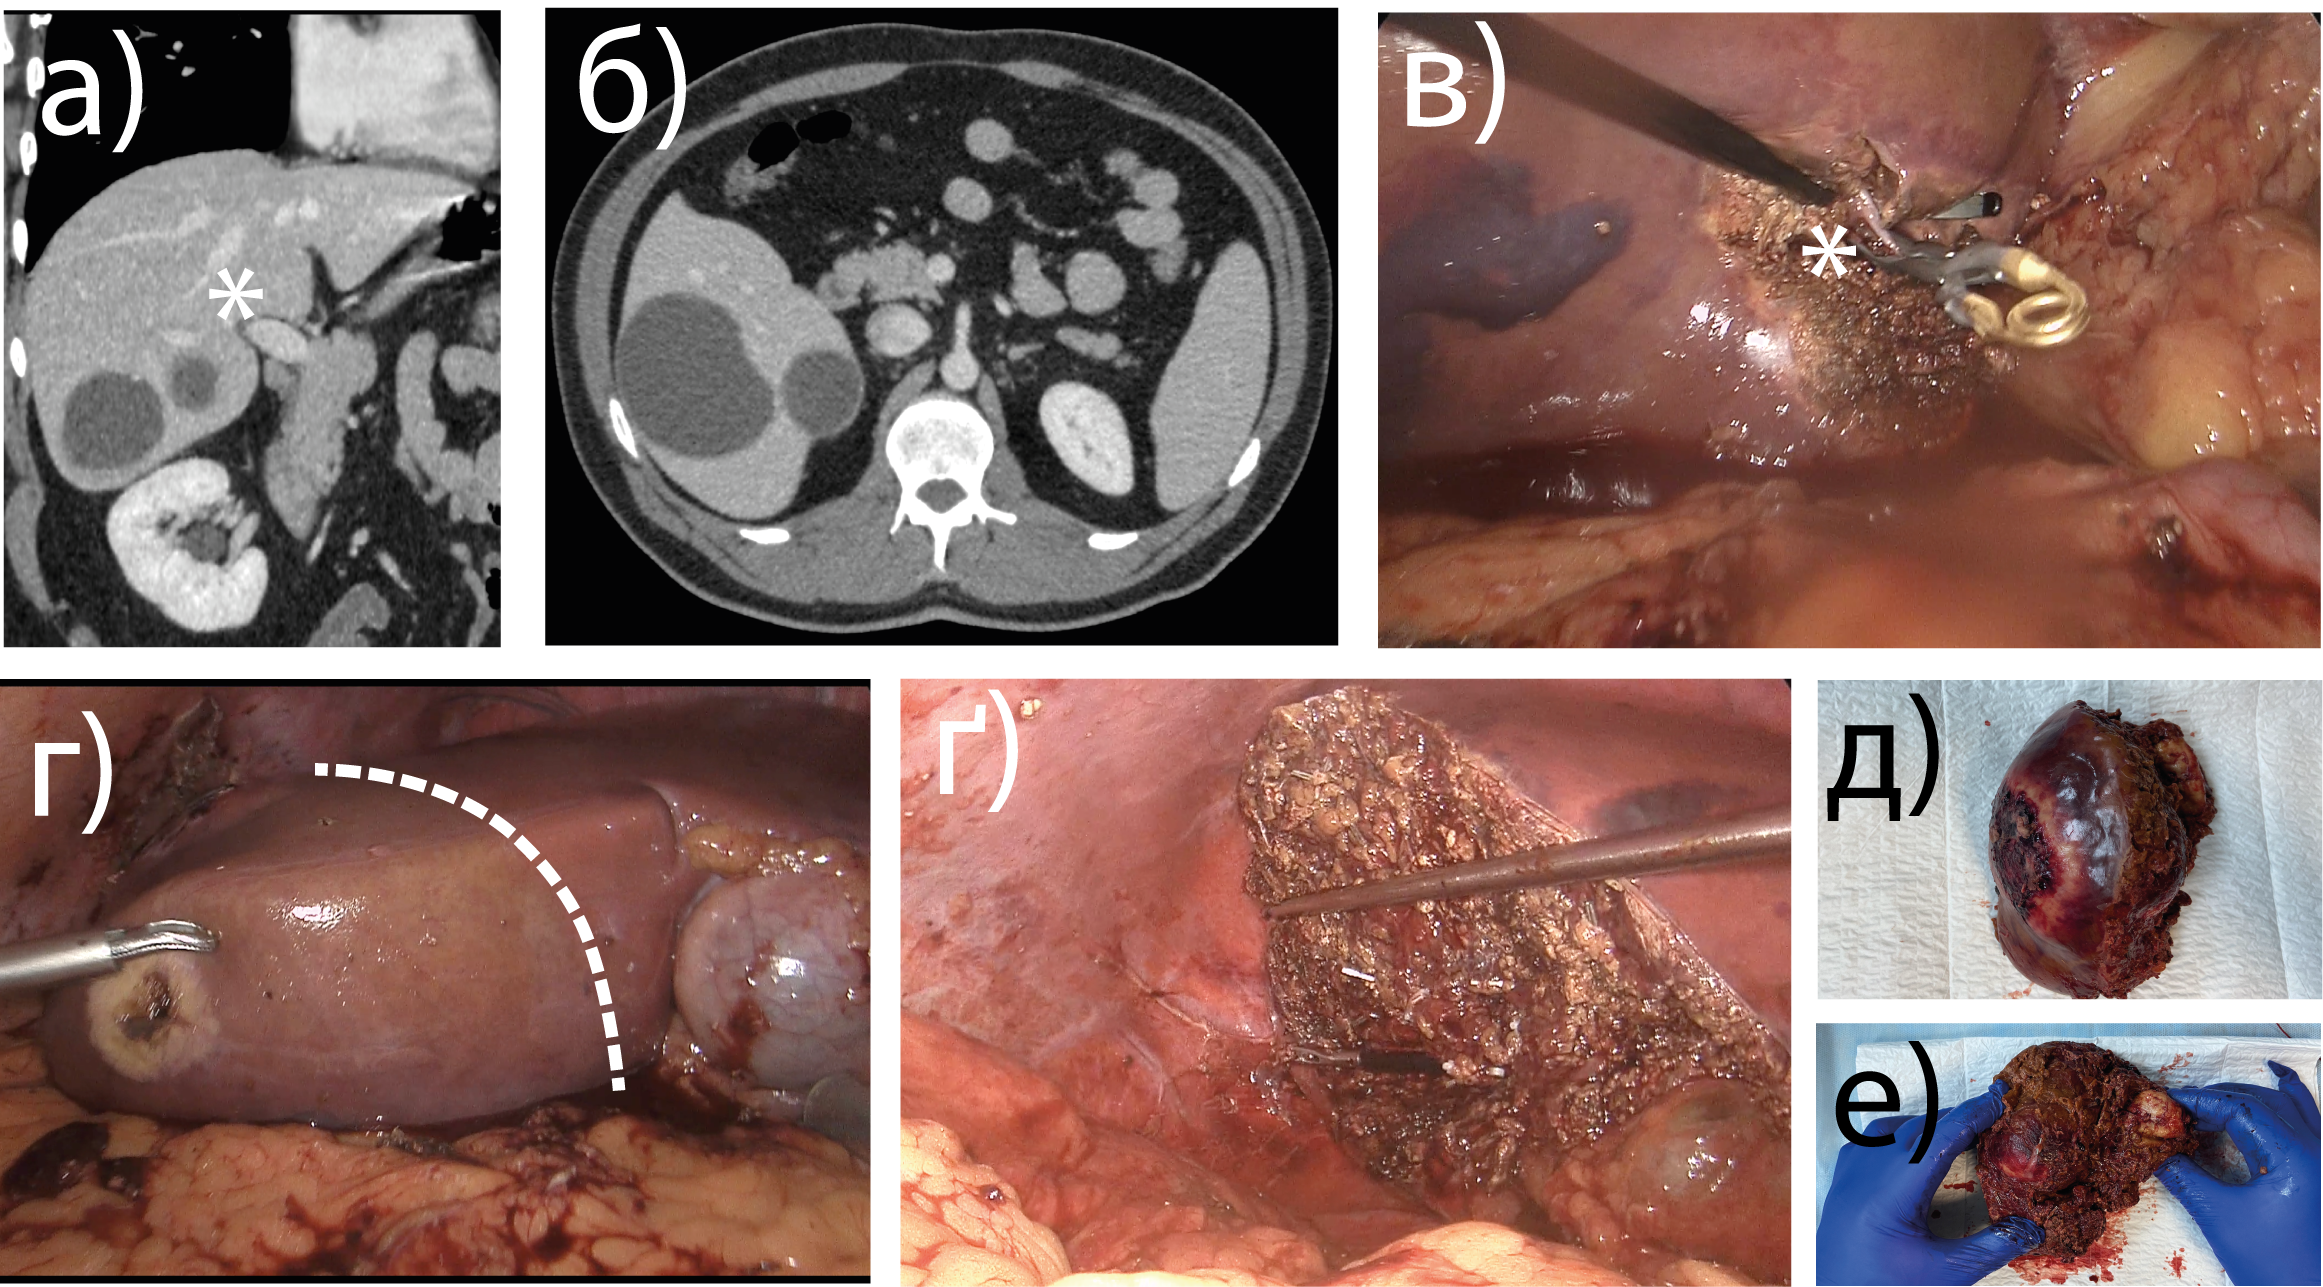
\includegraphics[width=0.95\textwidth]{Illustrations/Chapter_01/ECC-Sg6.png}
%\label{fig:ECC-Sg6}

%\medskip
%\small
%а,б) Передопераційне \acrshort{ct}. Ехінококові кисти розташовані в Sg 6 печінки та прилягають до сегментарного глісону (помічено зірочкою) в) Глісон Sg 6 виділено та кламповано г) Лінія демаркації після перетискання глісонової ніжки ґ) Площина резекції д,е) Макропрепарат  

%\end{figure}



Анатомічна радикальна резекція печінки є методом вибору для лікування більш агресивної форми паразитарного ураження печінки - альвеолококозу. За данними нещодавнього метааналізу \acrshort{llr} є потенційно ефективними методом лікування цього захворювання при дотриманні показів, а його результати порівняні із виконанням відкритих втручаннь \cite{Salm2019}. 

\subsubsection{Первинний внутрішньопечінковий холелітіаз}

Первинний внутрішньопечінковий холелітіаз (\acrshort{pil}) є хронічним захворюванням, більш ендемічним для східноазіатських країн, проте може зустрічатись і в європейських країнах. Захворювання може проявляти себе больовим синдромом або періодичними симптомами холангіту. Для корректного визначення способу лікування потрібно диференційювати \acrshort{pil} із вторинним холелітіазом, який може бути наслідком міграції конкрементів з жовчного міхура або наслідком попередніх гепатобіліарних втручаннь. Механізм виникниння \acrshort{pil} чітко не з'ясований, але відомо, що у європейського населення він часто асоційований з 4 типом кіст біліарного дерева (хворобою Каролі), яка є показом до трансплантації печінки. Також відомо, що \acrshort{pil} частіше локалізується в лівій долі печінки, що пов'язують із більшим кутом лівого дольового протоку до холедоху та сповільнення пасажу жовчі в ньому \cite{Giuliante2015}.

Показано хороші результати застосування \acrshort{llr} для \acrshort{pil}, особливо при найбільш частій лівобічній локалізації. Так доступні результати південнокорейського порівняльного дослідження результатів лікування \acrshort{pil}. У дослідження були включені 149 пацієнтів із \acrshort{pil}, яким було виконано резекцію печінки відкритим та лапароскопічним шляхом, на основі аналізу результатів лікування яких автори дійшли висновку, що \acrshort{llr} є радикальним та безпечним методом лікування, який дозволяє знизити післяопераційну морбідність та асоційований із скороченням періоду реабілітації.

\section{Лапароскопічний погляд на хірургічну анатомію печінки}

Лапароскопічна хірургія має відмінності у візуалізації порівняно із відкритою хірургією, які пов'язані із відображенням плоскої, спотворенної заломленням світла при проходженні крізь оптичну частину лапароскопа проекції тривимірного зображення на екран. Такі відмінності зумовлюють особливий вигляд анатомічних структур та затруднюють їх ідентифікацію відносно звичних орієнтирів. Розуміння принципів виникнення таких особливостей є основою для безпечного виконання \acrshort{llr}. У цьому підрозділі ми розглянемо сучасні погляди на анатомічну будову печінки та особливості її лапароскопічної візуалізації.

\subsection{Сучасна номенклатура хірургічної анатомії печінки}

Резекційна хірургія печінки в теперішньому вигляді не була б можливою без детального уявлення про її внутішню анатомічну будову. Сучасні знання про анатомію печінки базуються на работах Healey J., Schroy P. і Couinaud С., які розробили принципи сегментарного поділу печінки. В класифікації Couinaud С., печінка поділяється на ліву та праву напів-печінку, кожна з яких в свою чергу ділеться на медіальний та латеральний сектори по ходу лівої та правої печінкових вен \cite{COUINAUD1954}. Кожен з секторів, окрім лівого латерального далі поділяється на два сегменти. Першим сегментом (Sg I) печінки є каудальна доля, яка має автономне кровопостачання. Враховуючи каудальну долю загальна кількість сегментів по Couinaud складає 8 (у більш пізній версії класифікації автор виділив хвостатий відросток Sg I у окремий 9-й сегмент) і вони мають нумерацію по ходу годинної стрілки за анологією з районами Парижу. Кожен сегмент за Couinaud - це ділянка паренхіми печінки, яка має автономне кровопостачання та жовчовідтік за рахунок гілок глісонів третього порядку. 

\begin{figure}[h]
\caption{Сегментація печінки за C.Couinaud.}

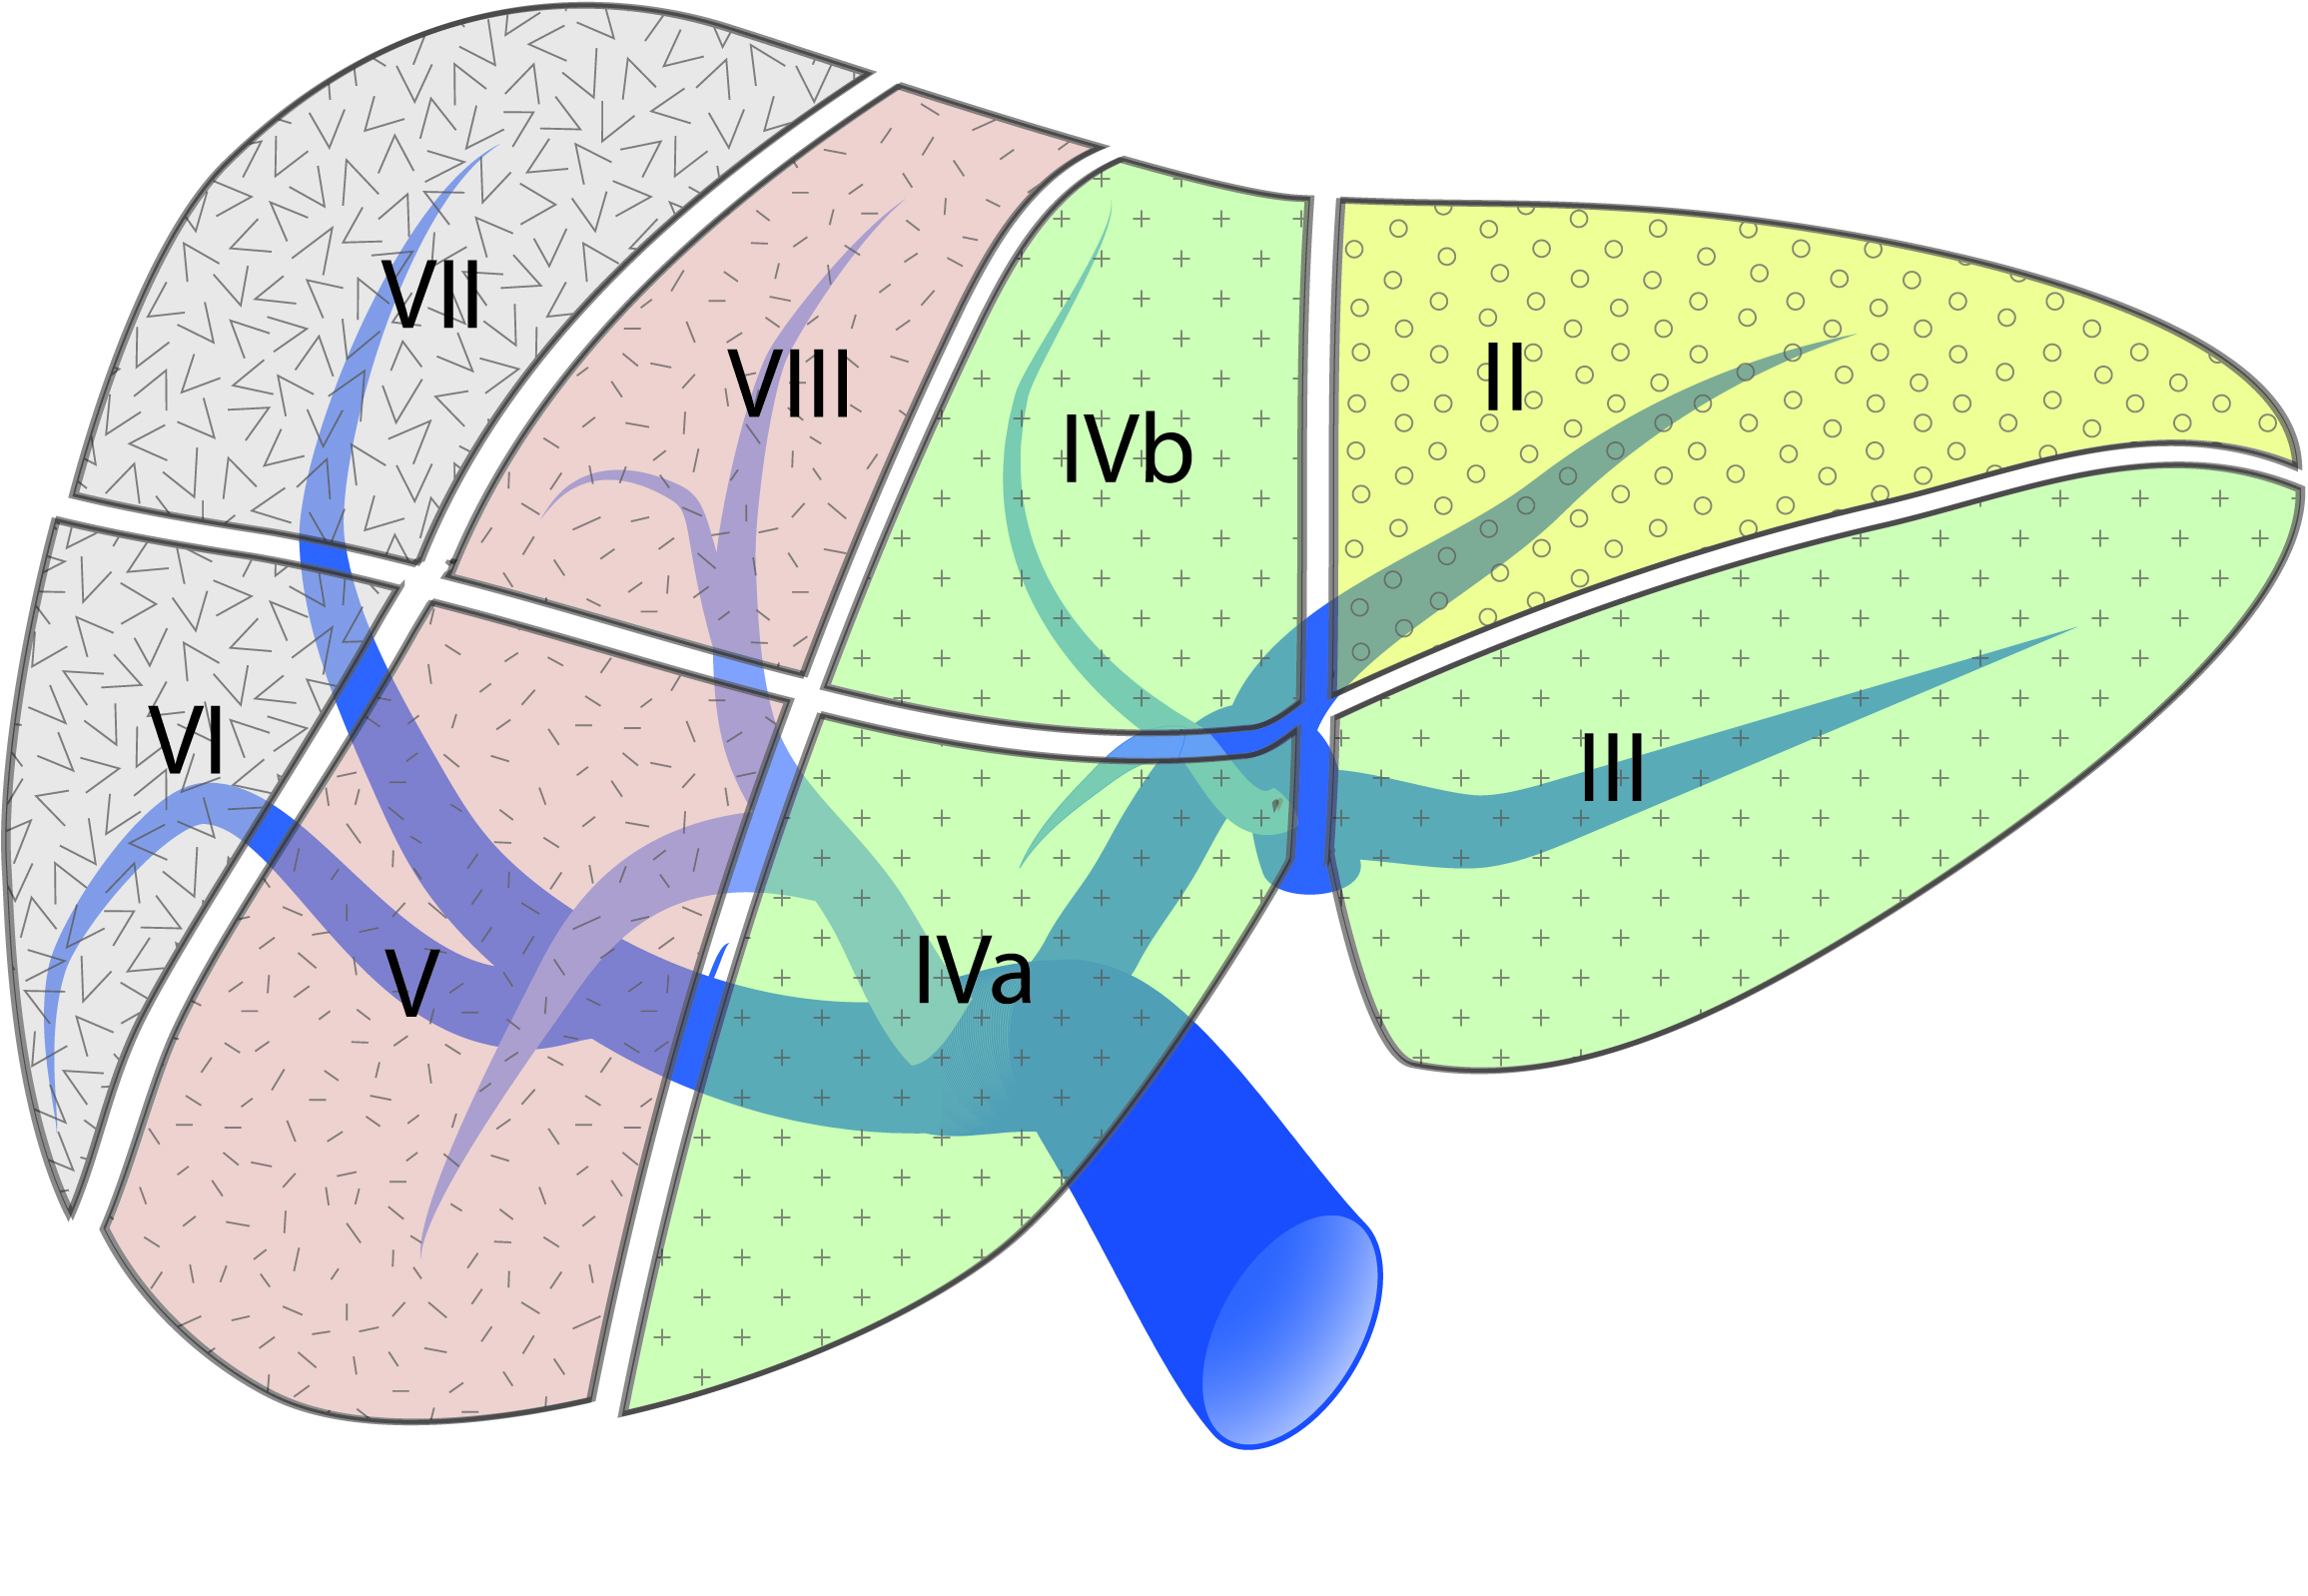
\includegraphics[width=0.9\textwidth]{Illustrations/Chapter_01/Couinaud.jpg}
\label{fig:Couinaud}

\medskip
\small
С. Сектори позначені окремими візерунками, сегменти позначені окремими контурами та римськими цифрами. Каудальна доля на малюнку не відображена. Синім кольором зображена ворітна вена.

\end{figure}

Класифікація Healey J. та Schroy P. використовує подібний принцип поділу, але на відміну від класифікації Couinaud поділяє печінку на ліву та праву долі, що діляться на сегменти (аналог секторів за Couinaud), які в свою чергу діляться на ділянки (аналог сегментів за Couinaud) \cite{HEALEY1953}. Принципово в цих двох класифікаціях відрізняється принцип поділу лівої долі печінки, яку Couinaud поділяє на сектори за ходом ворітної вени (до медіального сектору віднесено Sg 3, 4 а до латерального -  Sg 2), а Healey на сегменти за ходом жовчних шляхів та печінковї артерії (до медіального сегменту віднесено Sg 4 а до латерального - Sg 2,3).  

\begin{figure}[h]
\caption{Сегментація печінки за Healey J. та Schroy P.}

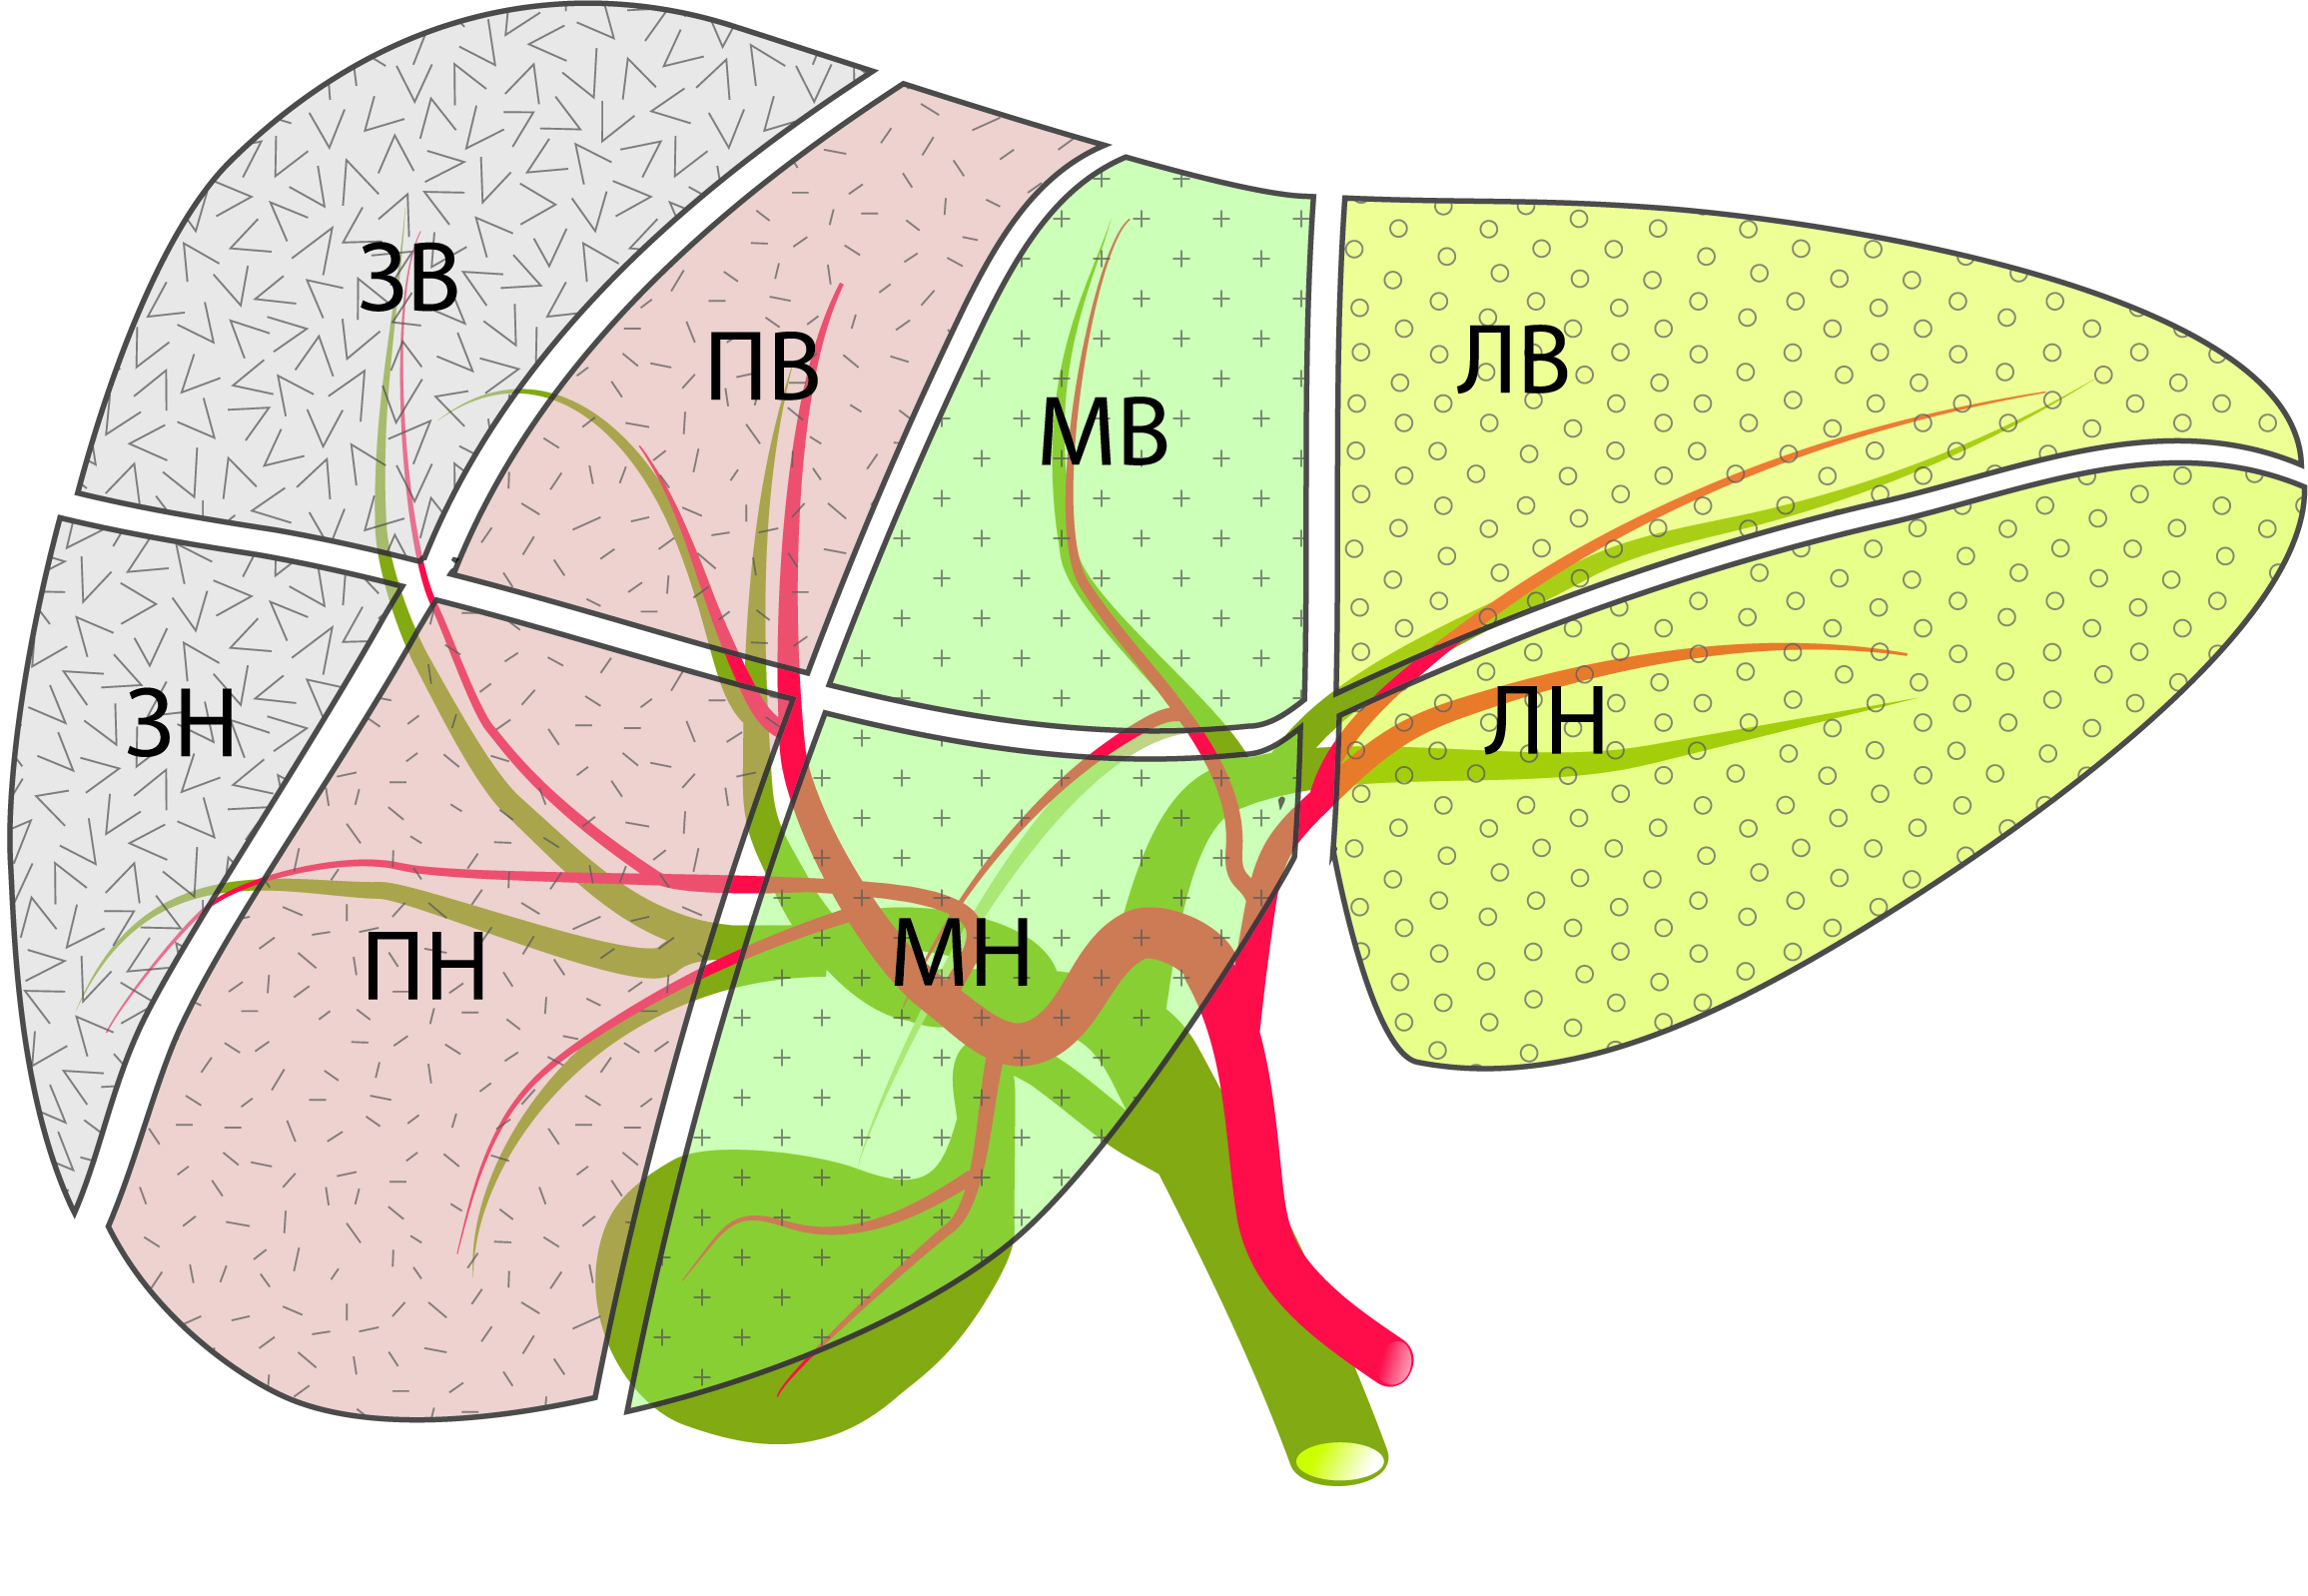
\includegraphics[width=0.9\textwidth]{Illustrations/Chapter_01/Healey.jpg}
\label{fig:Healey}

\medskip
\small
Сегменти позначені окремими візерунками, ділянки позначені окремими контурами скороченнями: ЛВ - латеральня верхня, ЛН - латеральна нижня, МВ - медіальна верхня, МН - медіальна нижня, ПВ - передня верхня, ПН - передня нижня, ЗВ - задня верхня, ЗН - задня нижня ділянка. Зеленим та червоним кольором зображені жовчні протоки та печінкова артерія відповідно.
\end{figure}

Так, як обидві класифікації мають широке розповсюдження в світі, з метою стандартизації на погоджувальній конференції в Брісбані у 2000 році Міжнародною Гепатопанкреатобіліарною Асоціацією було запропоновано універсальну номенклатуру для визначення анатомічних областей та видів резекцій печінки \cite{Pang2000}. Брисбанська класифікація побудована на основі класифікації Couinaud із заміною терміну "сектор" на "секція", за виключенням будови лівої долі, де Sg 2,3 віднесені до лівої латеральної секції. Згідно цієї класифікації таким анатомічним зонам, як напів-печінка (доля), секція та сегмент відповідають операції гемігепатектомія, секцієектомія та сегментектомія. Для уникнення термінологічних розбіжностей у цьому виданні ми будемо користуватись виключно номенклатурними термінами відповідно Брісбанській класифікації 2000 року.

\begin{figure}[h]
\caption{Брісбанська классифікація 2000 року номенклатури резекцій печінки}
\centering
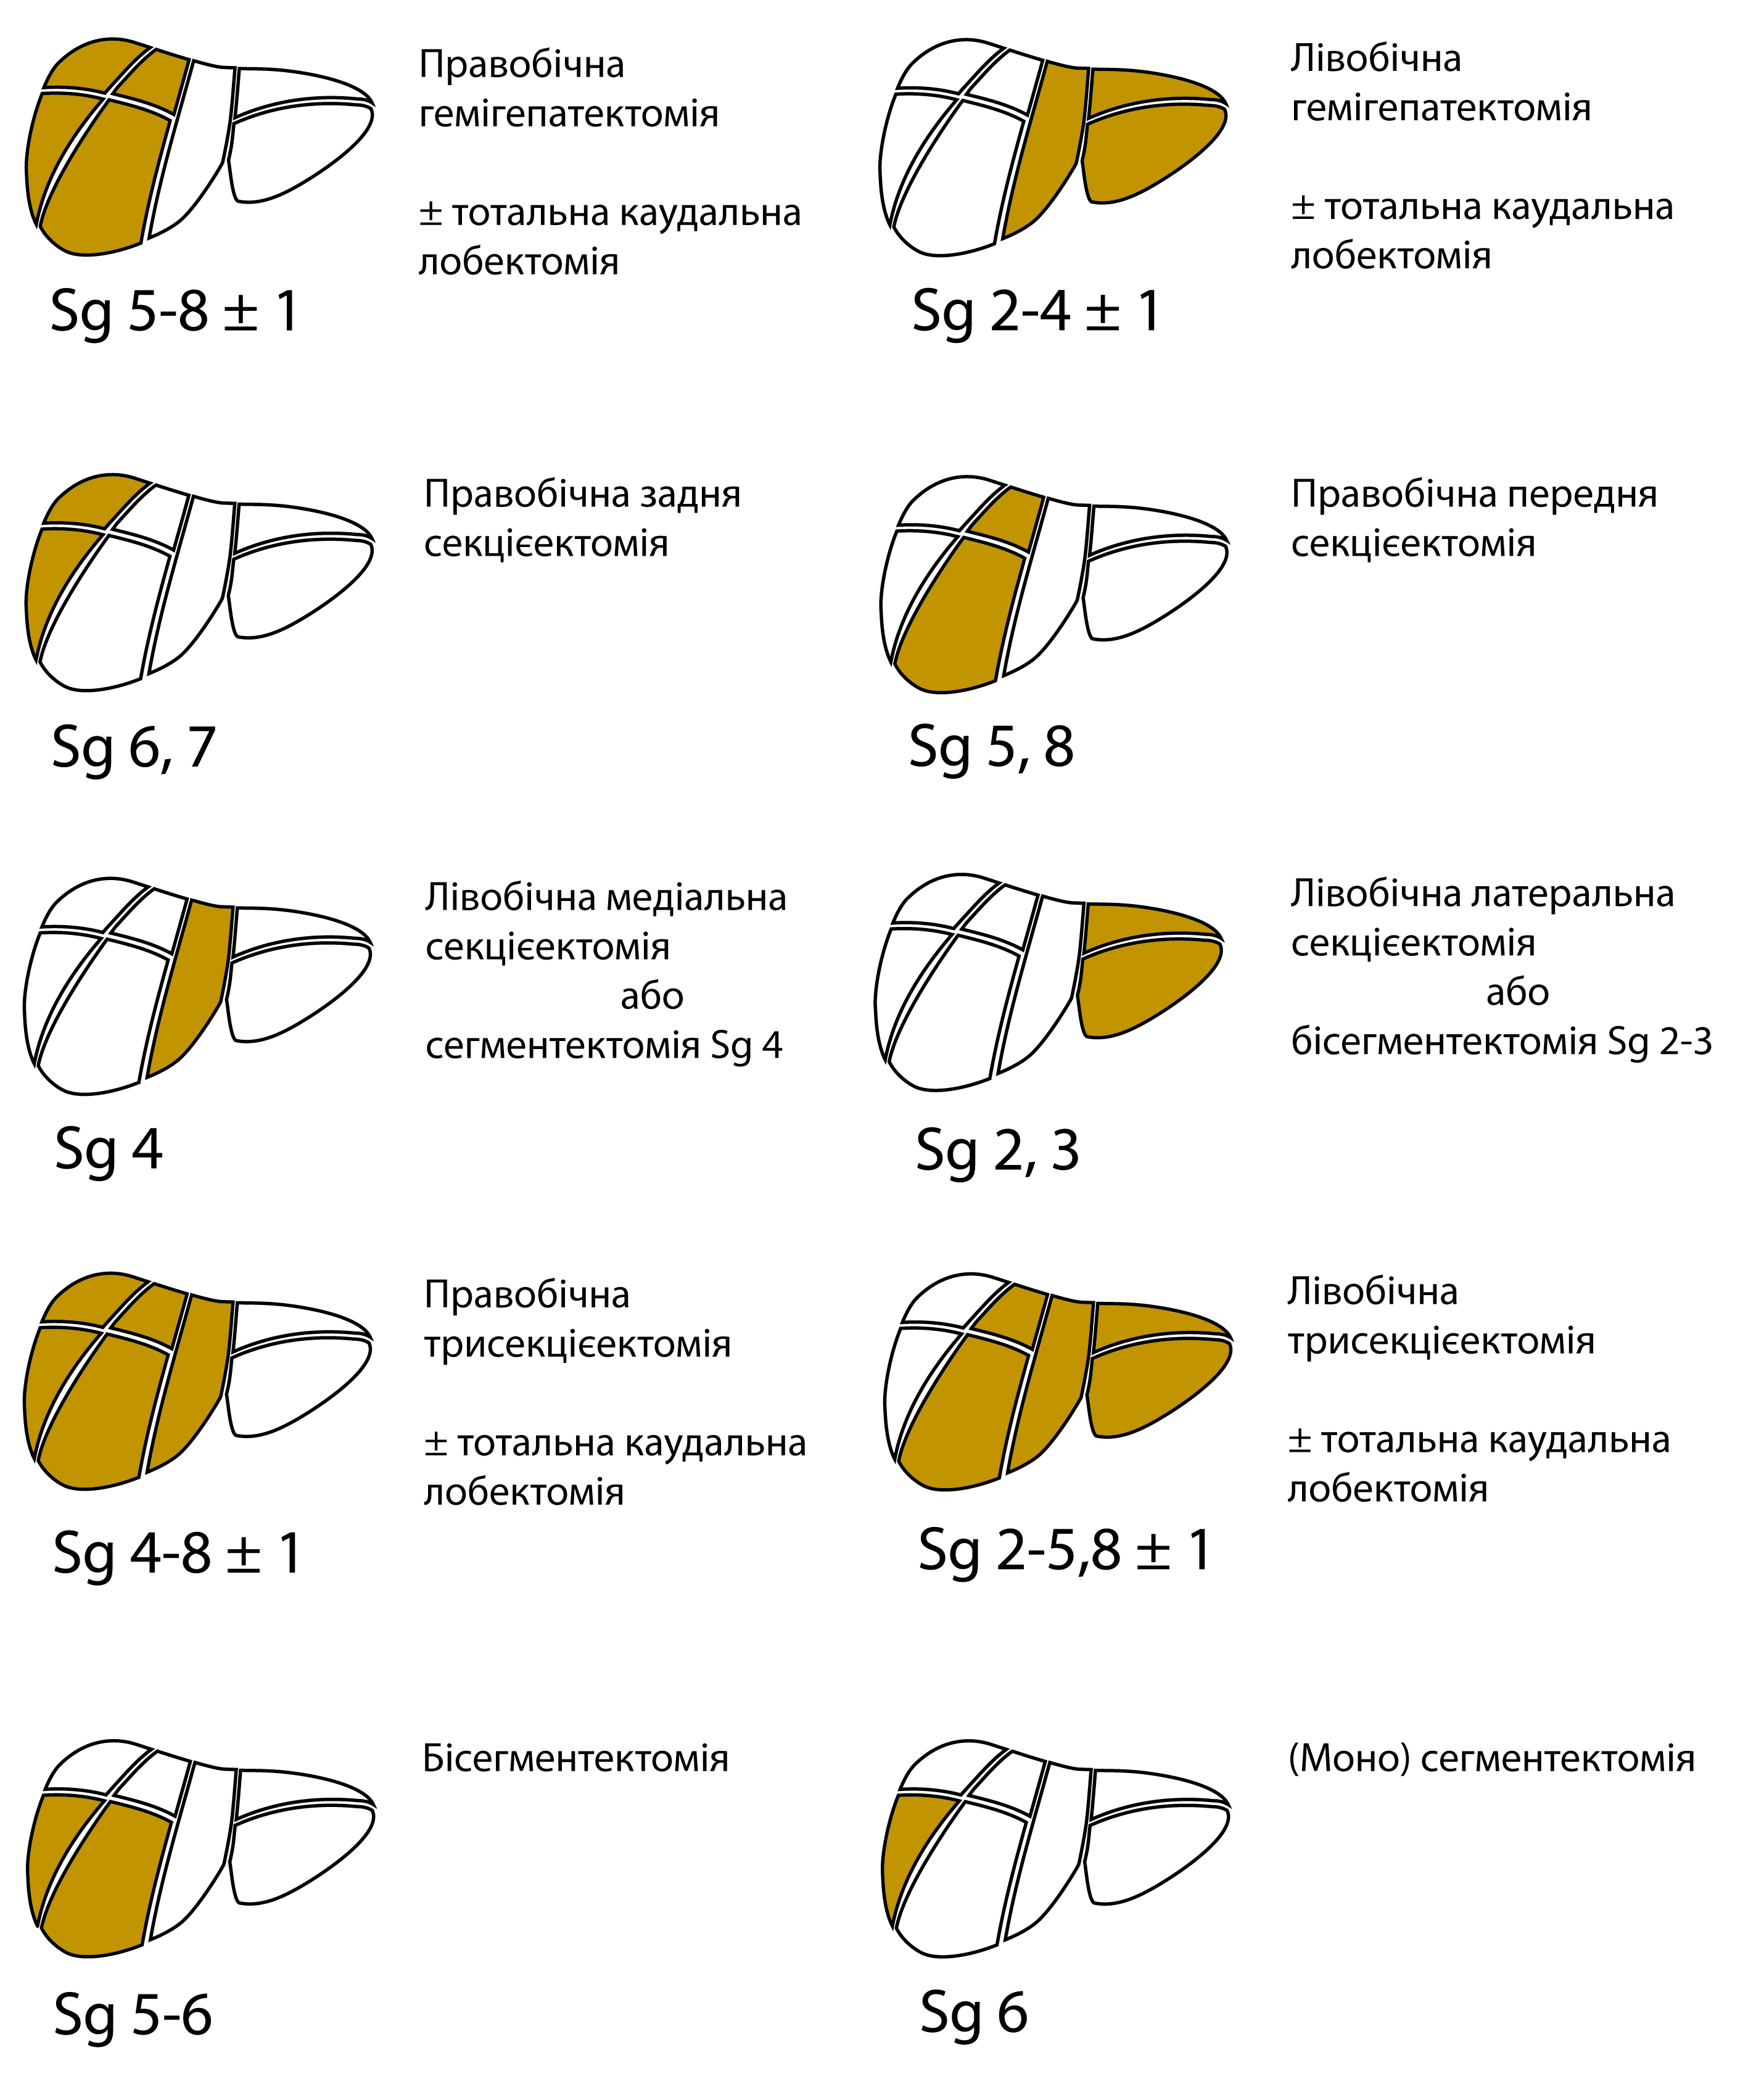
\includegraphics[width=0.9\textwidth]{Illustrations/Chapter_01/Brisbane.jpg}
\label{fig:Brisbane}
\end{figure}

\subsection{Лапароскопічна візуалізація зовнішніх орієнтирів}

На геометрію лапароскопічного зображення впливають кут огляду, кут напрямку зору та відстань до об'єкту. Скошена оптика (із кутом напрямку зору 30 та 45 градусів) дозволяє зробити огляд з різних боків, проте має більший ступінь спотворення зображення. Окрім того обмежений робочий простір, створений карбоксиперитонеумом, робить утрудненою візуалізацію цілого органу.

\subsubsection{Зв'язковий апарат}

Печінка вкрита очеревиною зі всіх боків, окрім невеликої частини  де очеревина переходить на діафрагму та формує коронарну зв'язку, яка далі переходить в ліву та праву трикутні зв'язки які разом утворюють її фіксуючий апарат. Серповидна зв'язка йде сагітально по серединній лінії від пупка та містить круглу зв'язку в свому вільному краї. Кругла зв'язка прямує до умбілікальної фіссури по вісцеральній поверхні лівої долі печінки, де входить в печінку та закінчується облітерованою частиною умбілікальної порції лівої ворітної вени. 

Серповидна зв'язка є чітким лапароскопічним орієнтиром, що відмежовує ліву латеральну секцію від інших сегментів печінки. Ліва трикутна зв'язка повністю доступна огляду по задньому краю Sg 2 печінки. Для візуалізації нижнього краю правої трикутної зв'язки необхідно підняти праву долю печінки. Верхній край правої трикутної зв'язки майже не доступний візуалізації без попередньої мобілізації її нижнього краю та коронарної зв'язки. 

\subsubsection{Структури печінково-дванадцятиперсної зв'язки}

В складі печінково-дванадцятиперсної зв'язки (\acrshort{pdl}) в печінку входять ворітна вена, печінкова артерія, гілки блукаючого нерва, а виходять жовчні та лімфатичні протоки. Структури \acrshort{pdl} покриті жировою та сполучною тканиною і шаром очеревини, яка переходить в малий сальник по лівому краю зв'язки. Пряма лапароскопічна візуалізація структур \acrshort{pdl} без диссекції можлива лише частково, як правило у пацієнтів з малою кількістю інтраабдомінальної жирової тканини. Зовнішніми орієнтирами є шийка жовчного міхура, отвір Вінслоу та малий сальник. Після холецистектомії сають доступними до візуалізації проекції правих переднього та заднього глісонів та глісону каудального відростку Sg 1. 

\begin{figure}[h]
\caption{Вхідні "ворота" капсули Лаенека}

\includegraphics[width=0.9\textwidth]{Illustrations/Chapter_01/External landmarks.png}
\label{fig:External_landmarks}

\small
Ворота позначено червоними ділянками та римськими цифрами I-VI.
\end{figure}


\subsection{Капсула Лаенека та концепція «вхідних воріт» для глісонового підходу}

Вперше описана Laennec в 1802 р. власна капсула печінки є тонкою мембраною, яка лежить субсерозно та на відміну від очеревини покриває цілий орган. Пізніше Couinaud була сформована концепція Глісонового плато - потовщеної фіброзної пластини, яка покриває судинно секреторні структури в складі Глісонових ніжок. Плато умовно ділять на три частини - хіларне, умбілікальне та міхурове, які переходять одне в інше. Також на основі гістологічних досліджень він довів, що капсула Лаенека не продовжується на Глісонові ніжки в складі хіларного плато, а йде окремим шаром вздовж усіх глісонових структур та печінкових вен, що входять в паренхіму печінки.

За сучасними уявленнями капсула Лаенека йде паралельно до глісонових структур, але в деякіх ділянках не прилягає до них щільно. Ця особливсість дає можливість безпечного хірургічного підходу до позапечінкового виділення Глісонових структур під час \acrshort{alr}, тому простір в місцях нещільного прилягання капсули Лаенека до глісонових гілок має назву "вхідних воріт" \cite{Sugioka2017}. Всього виділяють шість вхідних воріт для визначення яких є чотири анатомічних орієнтира - Аранцієва протока, умбілікальне плато, міхурове плато та Глісонова ніжка каудального відростка. Межею I воріт є каудальний кінець Аранцієвої протоки, II воріт - з'єднання між круглою зв'язкою та умбілікальним плато, III воріт - правий край лівого дольового глісону (Sg 2-4), IV воріт - лівий край правого переднього глісону, V воріт - біфуркація правих сегментарних глісонів, а VI воріт - простір між краєм заднього глісону та глісоном каудального відростку. 

\begin{figure}[h]
\caption{Вхідні "ворота" капсули Лаенека}

\includegraphics[width=0.9\textwidth]{Illustrations/Chapter_01/Gates.jpg}
\label{fig:Gates}

\small
Ворота позначено червоними ділянками та римськими цифрами I-VI.
\end{figure}


Диссекція в цих анатомічних ділянках та послідовне з'єднання між собою сусідніх воріт дозволяє виконати позапечінкову ізоляцію будь якого глісону з метою наступного виконання анатомічної резекції. Усі вхідні ворота легко доступні для лапароскопичноъ візуалізації: ворота I - III безпосередньо, а ворота IV - VI після попередньої холецистектомії (мал №)

\subsection{Анатомічна будова Sg I печінки}

Перший сегмент печінки або каудальна доля це центродорзально розташована ділянка паренхіми, яка має незалежне кровопостачання та жовчевідтік. Анатомічно вона обмежена наступними структурами: по задньому краю запечінковим сегментом \acrshort{ivc}, по нижньому краю воротами печінки, по верхньому - устям правої та загальним устям лівої та серединної печінкових вен, по пердньому та правому краю - тканиною Sg 4-8, а по лівому має зовнішню поверхню, вкриту капсулою (Спігелєва доля), яка пролабує до малого сальника та обмежена Аранцієвим протоком. Відповідно до класифікації Kumon M. \cite{Kumon2017}, каудальна доля поділяється на три частини: 1) Спігелєва порція (доля),  2) Паракавальна порція, 3) Порція каудального відростка. Для прямої лапароскопічної візуалізації  доступна лише частина каудального відростка та спігелєва доля після розсічення малого сальника.

Каудальна доля має власні портальні гілки, які йдуть від біфуркації ворітної вени в дорзальному напрямку. Аналогічно до портальних гілок, каудальна доля має власні артеріальні гілки від лівої та правої печінкових артерій та жовчні протоки, що дренуються в області конфлюенся лівого та правого дольових жовчних протоків. Спігєлева доля та порція каудального відростка мають по одній власній печінковій вені а паракавальна порція - декілька коротких печінкових вен, які дренуються безпосередньо в \acrshort{ivc}. 

\begin{figure}[h]
\caption{Анатомія Sg1 печінки}
\centering
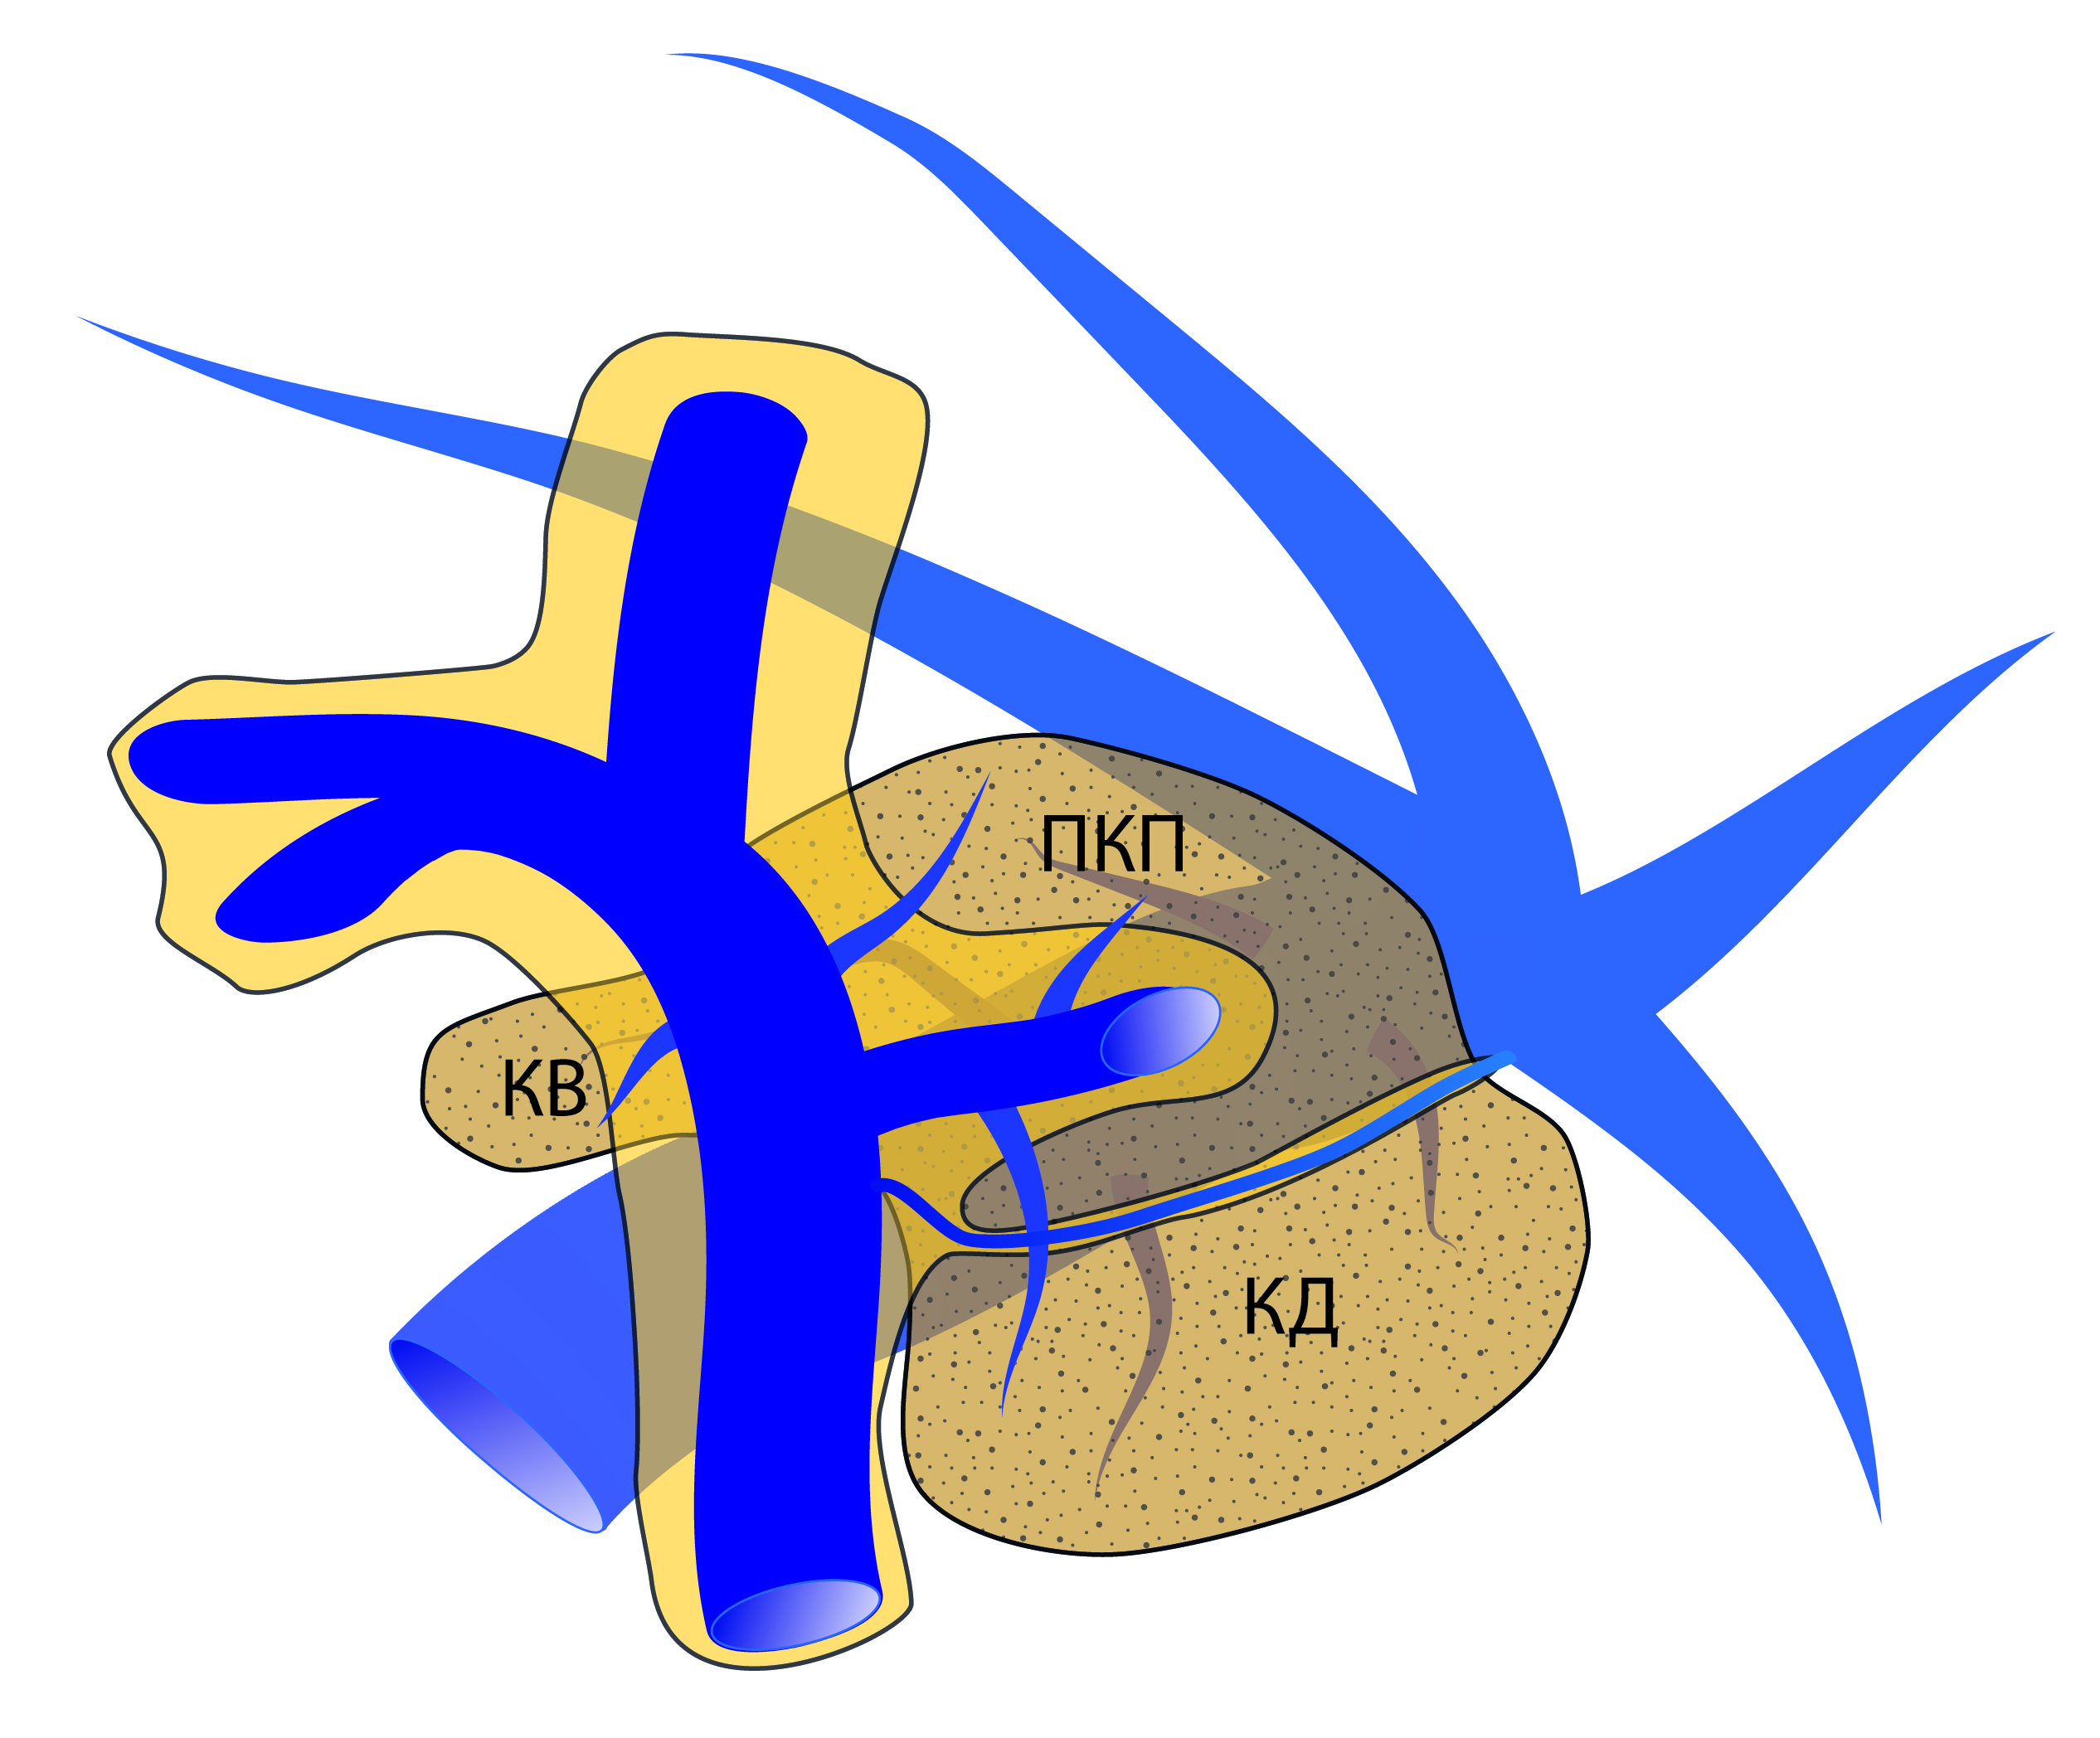
\includegraphics[width=0.9\textwidth]{Illustrations/Chapter_01/Sg1.jpg}
\label{fig:Sg1}
\end{figure}

\subsubsection{Нижня порожниста вена та печінкові вени}

Запечінковий сегмент \acrshort{ivc} інтимно прилягає до Sg 1 печінки звідки в нього дренуються короткі печінкові вени та обмежений згори окремим устям правої та загальним устям лівої та серединної печінкових вен. Для повної лапароскопічної візуалізації \acrshort{ivc} необхідна мобілізація правої трикутної та кронарної зв'язки та тракція правої долі печінки ліворуч.

\section{Імплементація методу лапароскопічної резекції печінки в практику}

Згідно рекомендацій третьої погоджувальної конференції в Саузхемптоні лапароскопічні резекції печінки рекомендовані до впровадження в центрах, що мають достатній досвід як резекційної печінкової так і лапароскопічної хірургії \cite{AbuHilal2017a}. Імплементація \acrshort{llr} повинна бути етапною, з поступовим збільшенням складності втручаннь. 

\subsection{Оцінка складності лапароскопічних резекцій печінки}
Для ефективного відбору пацієнтів на етапі імплементації необхідна об'єк\-тивна оцінка складності втручання. З цією метою запропоновано декілька систем, які прогнозують ризики розвитку ускладненнь після \acrshort{llr} \cite{Kawaguchi2018, Hasegawa2017a}. Найбільш широко вживана з цих систем, яка пройшла зовнішню валідацію, це IWATE-score (Таб.\ref{table:iwate}), названа так на честь префектури в Японії, де була розроблена \cite{Ban2014}. Система враховує локалізацію, розмір пухлини, близькість процесу до магістральних внутрішньопечінкових структур, необхідний об'єм резекції та  ступінь печінкової недостатності за Чайлдом. На основі оцінки цих факторів резекція оцінюється в балах складності від 1 до 10 (Таб.\ref{table:iwate-score}). Наявність 1-3 балів свідчить про низьку складність, 4-6 - середню складність, 7-10 - високу складність. 

% Складність LLR
\begin{table}
\begin{tabular}{ |p{0.15\linewidth} |p{0.05\linewidth} |p{0.05\linewidth}|p{0.05\linewidth}|p{0.05\linewidth}|p{0.05\linewidth}|p{0.05\linewidth}|p{0.05\linewidth}|p{0.05\linewidth}|p{0.05\linewidth}|p{0.05\linewidth}|p{0.05\linewidth}| }
 \hline
 \multicolumn{11}{|c|}{Складність \acrshort{llr}} \\
 \hline
 Бали & 1 & 2 & 3 & 4 & 5 & 6 & 7 & 8 & 9 & 10 \\
 \hline
 Складність   & \multicolumn{3}{p{0.15\linewidth}|}{Низька} & \multicolumn{3}{p{0.15\linewidth}|}{Середня} & \multicolumn{4}{p{0.20\linewidth}|}{Висока} \\
 \hline
 Визначення   & \multicolumn{3}{p{0.20\linewidth}|}{Для хірургів що починають \acrshort{llr} з досвідом до 10 операцій} & \multicolumn{3}{p{0.20\linewidth}|}{Для хірургів, що успішно виконють \acrshort{llr} низької складності з досвідом 10-50 операцій } & \multicolumn{4}{p{0.25\linewidth}|}{Для хірургів, що успішно виконють \acrshort{llr} середньої складності з досвідом більше 50 операцій } \\
 \hline
\end{tabular}

\caption{\label{table:iwate}Індекси IWATE для оцінки складності \acrshort{llr} }
\end{table}





% Бали складності
\begin{table}
\begin{tabular}[t]{ |p{0.5\textwidth}| p{0.3\textwidth}|  }
\hline
    \textbf{Локалізація ураження} & \textbf{Розмір ураження} \\

\multirow{6}{*}{
   % \rule{0pt}{100pt}   % Висота строки 
    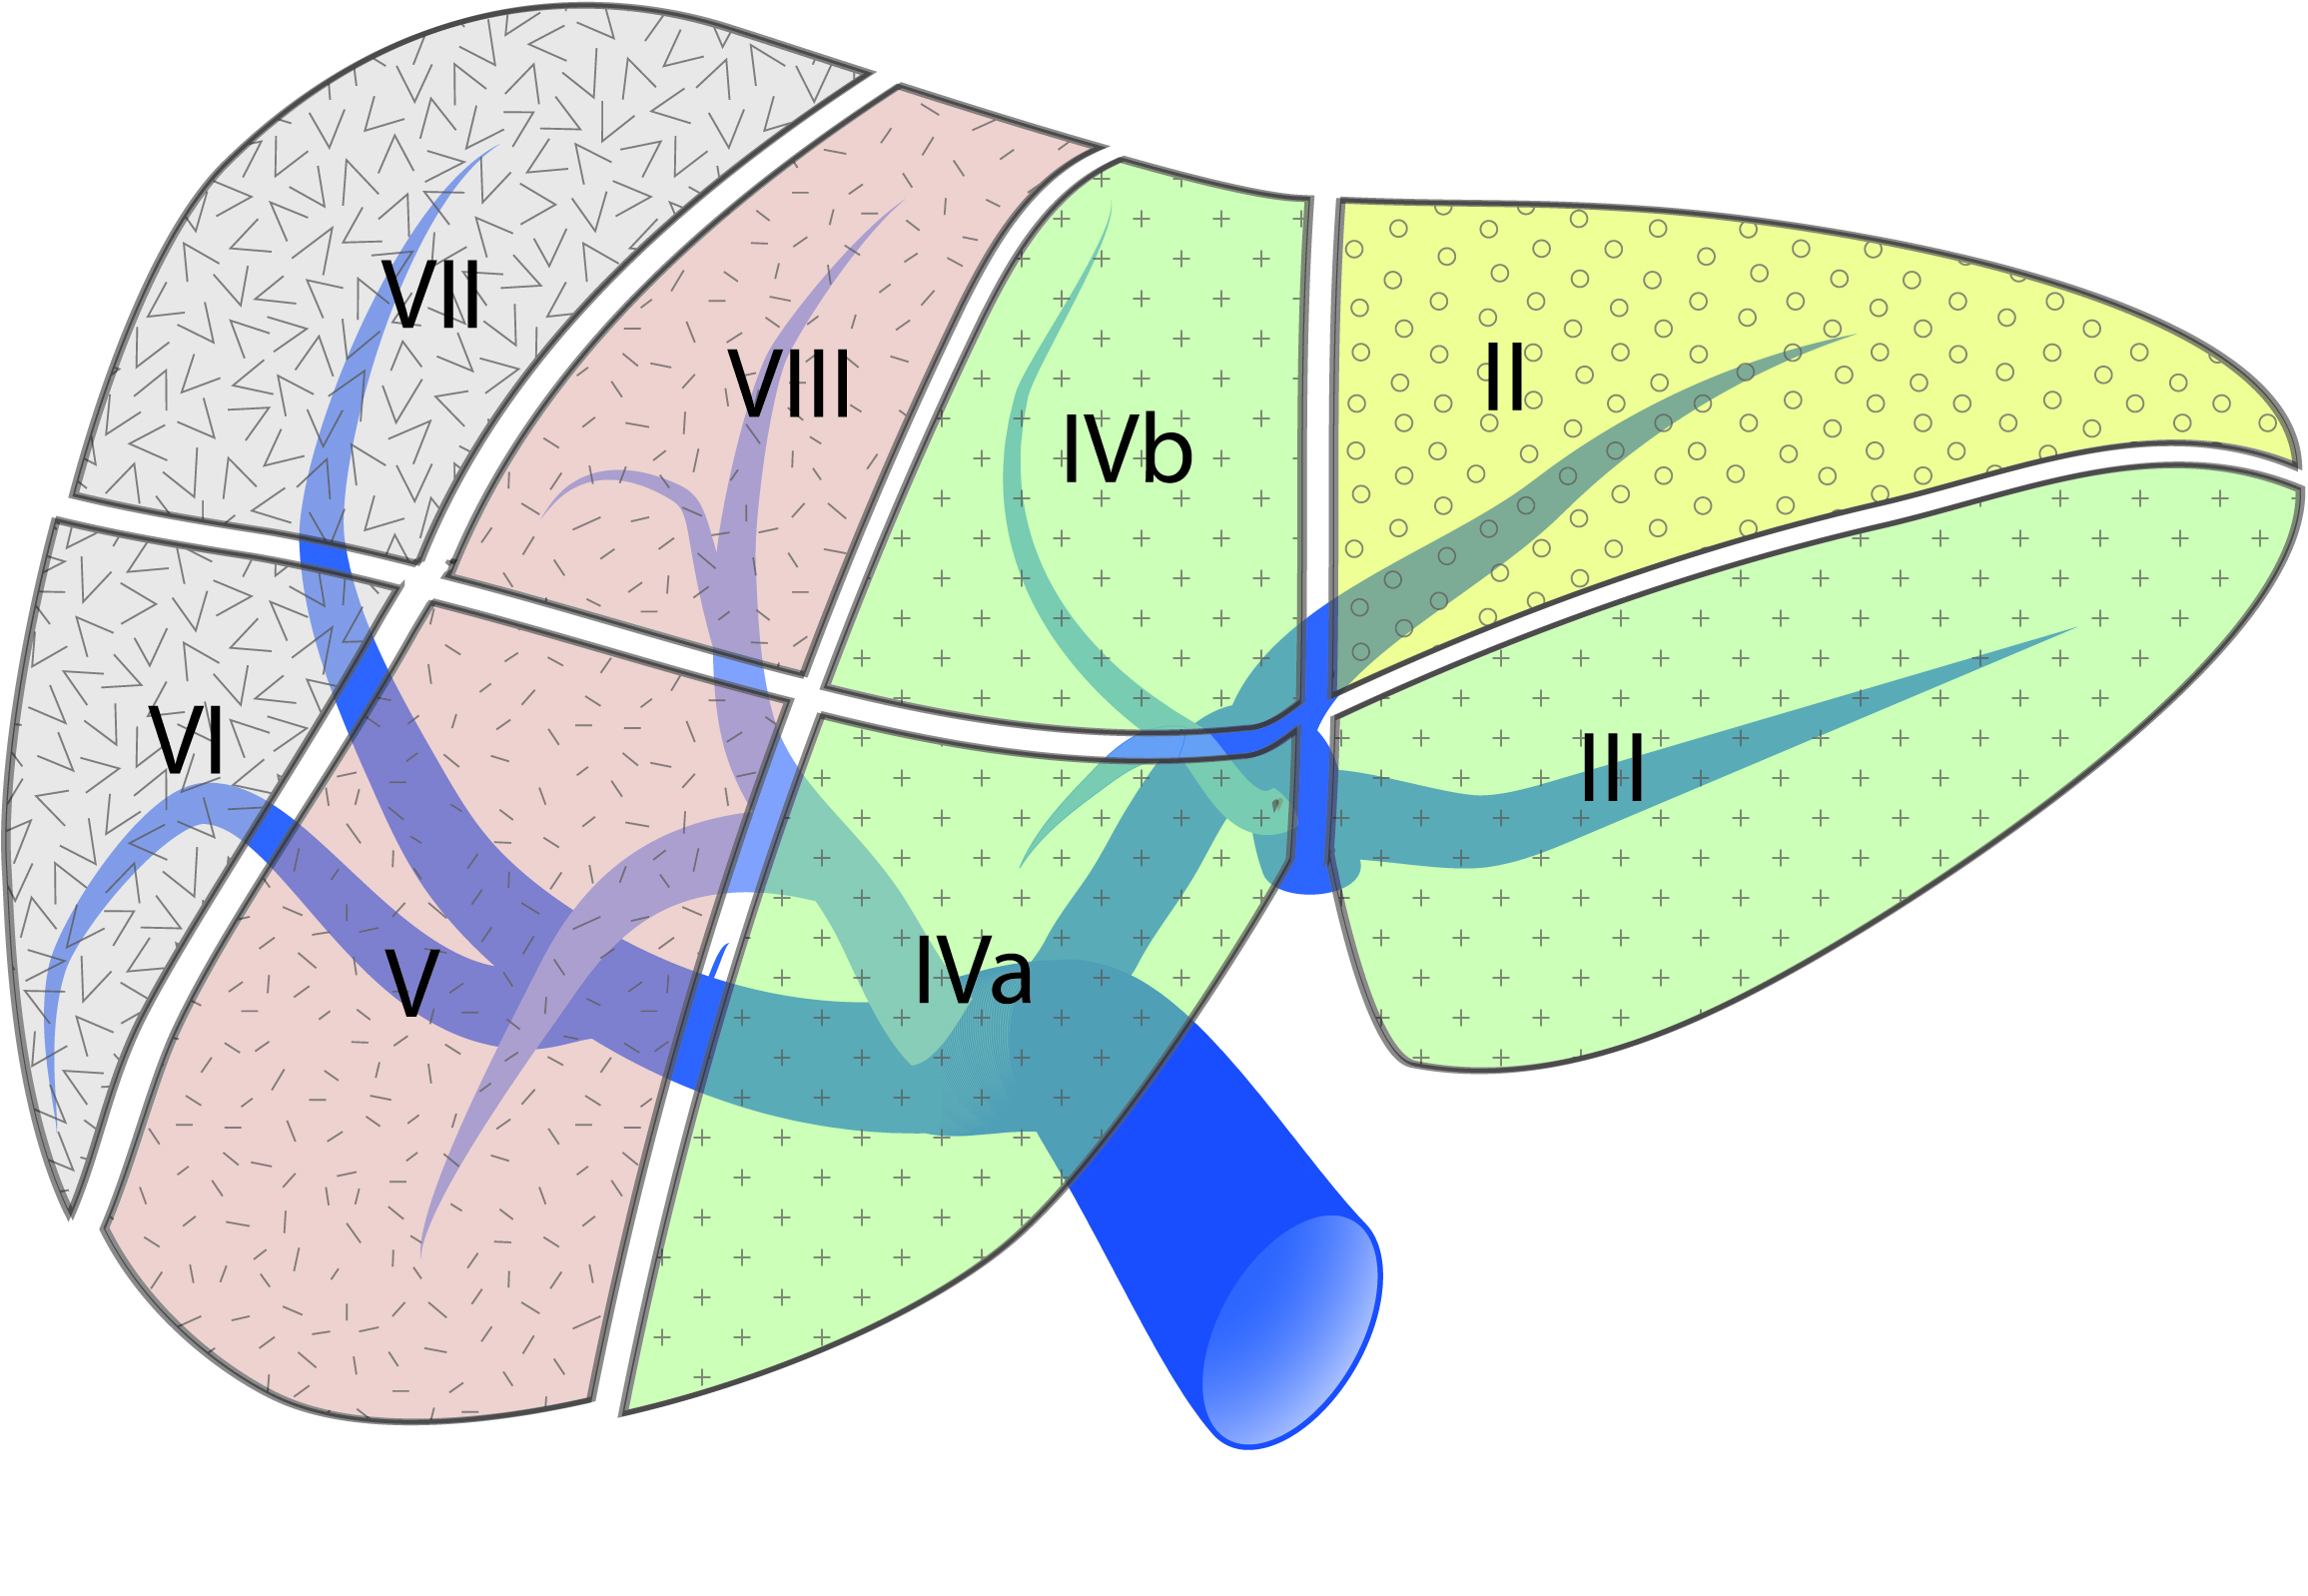
\includegraphics[width=0.3\textwidth]{Illustrations/Chapter_01/Couinaud.jpg} 
     \begin{tabular}{c|c} 
        Sg & Бали \\ %[0.5ex] 
        \hline\hline
        2 & 2 \\ 
        3 & 1 \\ 
        4 & 3 \\ 
        5 & 3 \\ 
        6 & 2 \\ 
        7 & 5 \\ 
        8 & 5 \\ 
     \end{tabular}
   }
 & \begin{centre}
    \begin{tabular}[t]{c c} 
      & Бали \\
      <3 см & 0 \\ 
     \geq 3 см & 1 \\ 
     
    \end{tabular}
  \end{centre} \\
 & \textbf{Близькість до судин} \\ 
 & \begin{centre}
    \begin{tabular}{c c} 
      & Бали \\
      Відсутня & 0 \\ 
      Наявна & 1 \\ 
    \end{tabular}
  \end{centre} \\
  & \\
  & \\
  & \\
\hline  
\textbf{Об'єм резекції} & \textbf{Функція печінки} \\   

   \begin{centre}
    \begin{tabular}{c c} 
      & Бали \\
      Паціальна резекція & 0 \\ 
      \acrshort{llls} & 2 \\ 
      Сегментектомія & 3 \\ 
      Не менше секцієеткомії & 4 \\
    \end{tabular}
  \end{centre}  
& \begin{centre}
    \begin{tabular}{c c} 
      & Бали \\
      Child-Pugh A & 0 \\ 
      Child-Pugh B & 1 \\ 
    \end{tabular}
  \end{centre} \\
\hline                  
\end{tabular}
\caption{\label{table:iwate-score}Шкала IWATE складності \acrshort{llr} }
\end{table}

\subsection{Етапи впровадження лапароскопічних резекцій печінки}
Процес імплементації \acrshort{llr} повинен бути системним, а в процес навчання повинна бути залучена вся хірургічна бригада (оператори, асистенти, анестезіологи, операційні сестри). Крива навчання для малих резекцій печінки складає 60 випадків, а для великих цей показник складає 55 випадків. Проходження хірургічною бригадоб кривої навчання малих резекцій може знизити цей показник для великих резекцій. Враховуючи це, запровадження програми \acrshort{llr} має сенс лише в госпіталях, в яких виконується більше 50 відкритих резекцій на рік \cite{Vigano2009, Hasegawa2017, Marcel2016}. 
Основні етапи, що має пройти клініка при впровадженні програми наступні:

\begin{enumerate}
    
    \item \textbf{Теоретична підготовка та матеріально-технічне забезпечення.} На цьому етапі оцінюють потенційну потребу клініки в \acrshort{llr} та відповідно неї формують одну чи декілька хірургічних бригад. Після проходження персоналом стажування в клініках з великим об'ємом \acrshort{llr} та набуттям початкового досвіду формується перелік необхідного обладнання та інструментів. 
    
    \item \textbf{Проходження кривої навчання малих \acrshort{llr}.} Для проходження цього етапу відбирають пацієнтів із ураженнями антеролатеральних сегментів невеликого розміру, на значному віддаленні від магістральних структур. Для перших 10 втручаннь необхідні випадки із рівнем складності 1-3 балів за шкалою IWATE (як правило це крайові парціальні резекції вогнищ < 3 см у пацієнтів без циррозу). Починаючи із 11 випадку рекомендовано збільшувати складність до 4-6 балів за шкалою IWATE за ракунок анатомічних сегментектомій антеролатеральних сегментів та лівої латеральної секцієектомії. Мета цього етапу - відпрацювання базових елементів техніки \acrshort{llr} таких, як прийом Прінгла, мобілізація лівої та правої долей печінки, транссекція паренхіми, гемостаз, диссекція та лігування лівої печінкової вени.
    
    \item \textbf{Проходження кривої навчання великих \acrshort{llr}.} Після успішного проходження кривої навчання малих резекції (~ 60 випадків) переходять до виконання великих резекцій печінки (3 або більше суміжних сегменти), та підвищують поріг складності операцій до 7-10 балів за шкалою IWATE. Для цього підбирають випадки із утвореннями більшого розміру, включаючи локалізацію у правій долі та важкодоступних сегментах 7 та 8. На цьому етапі відпрацьовують такі складні елементи техніки \acrshort{llr} як  ізольована або гліссон-орієнтована диссекція правих портальних структур, диссекція запечінкового відділу \acrshort{ivc}, диссекція та лігування \acrshort{rhv}, транссекція паренхіми при великих новоутвореннях. Починають етап із виконання правобічних та лівобічних гемігепатектомій, потім переходять до секцієектомій та мезогепатектомій та при їх успішному опануванні виконують анатомічні резекції Sg 7 та 8. 
    
    \item \textbf{Введення \acrshort{llr} в стандарти надання допомоги клінікою.} Після проходження хірургічною бригадою кривої навчання \acrshort{llr} може бути закріплена в протоколі надання допомоги пацієнтам із вогнищевою патологією печінки як один з можливих методів. Для пацієнтів із ураженням антеролатеральних сегментів \acrshort{llr} є стандартом практики. Після імплементації \acrshort{llr} в сучасному відділенні гепатобіліарної хірургії high-volume центру їх доля як правило сягає 30-80\% від загального числа резекцій печінки. 

\end{enumerate}

\printbibliography[heading=subbibliography] 

\end{refsection}